
\documentclass[12pt,oneside]{article}

%%%%%%%%%%%%%%%%%%%%%%%%%%%%
%%   Zusaetzliche Pakete  %%
%%%%%%%%%%%%%%%%%%%%%%%%%%%%
\usepackage{enumerate}  
\usepackage{fancyhdr}
\usepackage{polynom}
\usepackage{a4wide}
\usepackage[utf8]{inputenc}
\usepackage{graphicx}
\usepackage{palatino}
\usepackage{python}
\usepackage{scrextend}
\usepackage{multirow}
\usepackage[toc,page]{appendix}
\usepackage{booktabs}
\usepackage{listings}
\usepackage{titlesec}
\usepackage{amsthm}
\usepackage{amssymb}
\usepackage{amsmath}
\usepackage[utf8]{inputenc}
\usepackage[options ]{algorithm2e}
\usepackage[ruled,vlined]{algorithm2e}
\usepackage{lmodern}
\usepackage[utf8]{inputenc}
\usepackage[english,german]{babel}
\usepackage{xcolor}
\usepackage{amsfonts}
\usepackage{etoolbox}
\usepackage[]{algorithm2e}
\usepackage{blindtext}
\usepackage{algorithm}
\usepackage[noend]{algpseudocode}
\usepackage{comment}
\usepackage[
backend=biber,
style=alphabetic,
sorting=ynt
]{biblatex}
\usepackage{enumitem}% http://ctan.org/pkg/enumitem

% for footnotes
\deffootnote[10pt]{10pt}{10pt}{\makebox[10pt][l]{\thefootnotemark\hspace{10pt}}}

% notendig für Definitionen und Theoreme
\newtheorem{theorem}{Theorem}[section]
\newtheorem{corollary}{Corollary}[theorem]
\newtheorem{lemma}[theorem]{Lemma}
\newtheorem{fact}[theorem]{Fakt}
\newtheorem{example}[theorem]{Beispiel}

\newtheorem{prop}{Proposition}[section]

\theoremstyle{remark}
\newtheorem*{remark}{Remark}

\theoremstyle{definition}
\newtheorem{definition}{Definition}[section]
%%%%%%%%%%%%%%%%%%%%%%%%%%%%%%

%folgende Zeile auskommentieren für englische Arbeiten
\usepackage[ngerman]{babel}
%folgende Zeile auskommentieren für deutsche Arbeiten
%\usepackage[ngerman, english]{babel}
\usepackage[T1]{fontenc}
\usepackage[utf8]{inputenc}
\usepackage[bookmarks]{hyperref}
\usepackage[justification=centering]{caption}
\usepackage[style=authoryear,natbib=true,backend=biber,maxbibnames=20]{biblatex}
\usepackage{csquotes}
\bibliography{literatur}
\addbibresource{literatur.bib}
\setlength{\parindent}{0em} 
\setlist[itemize]{noitemsep, topsep=0pt}
\setlist[enumerate]{noitemsep, topsep=0pt}


%%%%%%%%%%%%%%%%%%%%%%%%%%%%%%
%% Definition der Kopfzeile %%
%%%%%%%%%%%%%%%%%%%%%%%%%%%%%%

\pagestyle{fancy}
\fancyhf{}
\cfoot{\thepage}
\setlength{\headheight}{16pt}
\newcommand\showdiv[1]{\overline{\smash{)}#1}}
%%%%%%%%%%%%%%%%%%%%%%%%%%%%%%%%%%%%%%%%%%%%%%%%%%%%%
%%  Definition des Deckblattes und der Titelseite  %%
%%%%%%%%%%%%%%%%%%%%%%%%%%%%%%%%%%%%%%%%%%%%%%%%%%%%%

\newcommand{\JMUTitle}[9]{

  \thispagestyle{empty}
  \vspace*{\stretch{1}}
  {\parindent0cm
  \rule{\linewidth}{.7ex}}
  \begin{flushright}
    \vspace*{\stretch{1}}
    \sffamily\bfseries\Huge
    #1\\
    \vspace*{\stretch{1}}
    \sffamily\bfseries\large
    #2\\
    \vspace*{\stretch{1}}
    \sffamily\bfseries\small
    #3
  \end{flushright}
  \rule{\linewidth}{.7ex}

  \vspace*{\stretch{1}}
  \begin{center}
    
\includegraphics[width=4in]{logo} \\
    \vspace*{\stretch{1}}
    \Large  Bachelorarbeit   \\

    \vspace*{\stretch{2}}
   \large Lehrstuhl für Mathematik \\
    \large und Informatik \\
    \large Universität Leipzig\\
    \vspace*{\stretch{1}}
    \large Betreuer:  #8 \\[1mm]
    
    \vspace*{\stretch{1}}
    \large Leipzig, den #7
  \end{center}
}

\titlespacing*{\section}
{0pt}{3.5ex plus 1ex minus .2ex}{.2ex plus .2ex}
\titlespacing*{\subsection}
{0pt}{1.5ex plus 1ex minus .2ex}{.2ex plus .2ex}
\titlespacing*{\subsubsection}
{0pt}{1.5ex plus 1ex minus .2ex}{.2ex plus .2ex}

%%%%%%%%%%%%%%%%%%%%%%%%%%%%
%%  Beginn des Dokuments  %%
%%%%%%%%%%%%%%%%%%%%%%%%%%%%

\begin{document}

  \JMUTitle
      {Deterministischer Primzahltest mit polynomieller Laufzeit: Der AKS-Primzahltest}  
      {Salman Salman}                        
      {3753924}
      
      {Fakultät für Informatik und Mathematik}  % Name der Fakultaet
      {Leipzig 2020}                          % Ort und Jahr der Erstellung
      {\today}                              % Tag der Abgabe
      {Prof. Dr. Andreas Maletti}               % Name des Erstgutachters
      {Zweitgutachter}                          % Name des Zweitgutachters
      
  \clearpage

\lhead{}
\pagenumbering{Roman} 
    \setcounter{page}{1}

\tableofcontents
\clearpage

\addcontentsline{toc}{section}{\listfigurename}
\listoffigures

\addcontentsline{toc}{section}{\listtablename}
\listoftables
\clearpage

\setlength{\parskip}{0.5em} 


%%%%%%%%%%%%%%%%%%%%%%%%%%%%
%%  Kurzzusammenfassung   %%
%%%%%%%%%%%%%%%%%%%%%%%%%%%%
\lhead{Abstract}
\section*{Abstract}
Primzahlen haben in der Informatik, speziell im Anwendungsgebiet der Kryptographie, eine sehr hohe Relevanz für moderne kryptographische Systeme ist es von Wichtigkeit selbige schnell bestimmen zu können. Hierzu werden effiziente Algorithmen zur Lösung des Primalitätsproblems benötigt. Das Primalitätsproblem umfasst die Frage um die Entscheidung, ob eine gegebene Zahl eine Primzahl ist oder nicht. Der erste deterministische Primzahltest in Polynomialzeit wurde von den indischen Informatikern Agrawal, Kayal, und Saxena vorgestellt. Der nach ihnen benannte AKS-Algorithmus wird im Rahmen dieser Arbeit repräsentiert, implementiert und evaluiert.  


%%%%%%%%%%%%%%%%%%%%%%%%%%%%
%%  Einstellungen  %%
%%%%%%%%%%%%%%%%%%%%%%%%%%%%
\clearpage
\pagenumbering{arabic}  
    \setcounter{page}{1}
\lhead{\nouppercase{\leftmark}}

%%%%%%%%%%%%%%%%%%%%%%%%%%%%
%%  Hauptteil  %%
%%%%%%%%%%%%%%%%%%%%%%%%%%%%

 

\section{Einleitung} \label{einleitung}

\subsection{Gliederung der Arbeit}
Die Arbeit gliedert sich in sechs Bestandteile, wobei der
erste Teil die Einleitung darstellt. Dort wird ein Überblick in das Thema gegeben und die Zielsetzung der Arbeit definiert.

Das zweite Kapitel enthält die Grundlagen. Hier werden Begriffe und Konzepte erläutert, die für das weitere Verständnis der Arbeit eine Rolle spielen. 

Der Algorithmus und seine Korrektheit sind die Bestandteile des dritten Kapitels. Dort wird zunächst die Grundidee des AKS-Algorithmus erläutert. Danach wird der Algorithmus angegeben, dabei werden die Schritte des Algorithmus auch erklärt. Anschließend soll die Korrektheit des Algorithmus bewiesen. 

Im vierten Kapitel wird die mathematische Laufzeitanalyse des Algorithmus vorgestellt, dabei werden die Laufzeiten der einzelnen Schritte (STEPS 1-6) des AKS-Algorithmus ausführlich analysiert.

Das fünfte Kapitel beinhaltet die experimentelle Laufzeit- und Korrektheitsanalyse, dort  soll die Laufzeit der Schritte des Algorithmus auf einem Rechner getestet. Darüber hinaus soll auch die Korrektheit dieser Schritte geprüft. Schließlich soll der AKS-Algorithmus mit dem naiven Algorithmus\footnote{. Der naive Algorithmus ist der beste nicht probabilistische Algorithmus. Die Laufzeit dieses Algorithmus ist $\Omega(\sqrt{n})$} verglichen werden, um zu zeigen, dass der AKS-Algorithmus eine bessere Laufzeit hat.  

\subsection{Überblick}
Eine Primzahl ist eine von 1 verschiedene natürliche Zahl, die keine Teiler außer 1 und sich selbst hat. Die Frage, ob eine Zahl eine Primzahl ist oder nicht, war schon im antiken Griechenland interessant. Euklid hat sich mit dieser Frage beschäftigt und bewiesen, dass es unendlich viele Primzahlen gibt. Im 3. Jahrhundert v. Chr. hat der griechische Mathematiker Eratosthenes einen Algorithmus zur Bestimmung einer Liste aller Primzahlen kleiner oder gleich einer vorgegebenen Zahl vorgestellt. Sein Algorithmus ist jedoch zur Lösung des Primalitätsproblem nicht effizient, da die Generierung solcher Listen bei sehr großen Zahlen zu aufwendig wird.

Im 17. und 18. Jahrhundert haben Wissenschaftler nach einem Verfahren zum Finden von Primzahlen gesucht. Ein wichtiges Resultat war der Satz von Wilson, der britische Mathematiker John Wilson(1741-1793) hat einen Satz aufgestellt, um Primzahlen von zusammengesetzten Zahlen zu unterscheiden. Der Satz lautet: $p \geq 2$ ist genau dann eine Primzahl, wenn $(p - 1)! + 1$ durch $p$ teilbar ist. Der französische Wissenschaftler Marin Mersenne(1588 - 1648) hat sich auch mit Primzahlen beschäftigt, er behauptete, dass für eine nach ihm benannte mersennsche Zahl(eine Zahl der Form $2^p - 1$) genau dann eine Primzahl, wenn $p$ eine Primzahl ist. Seine Behauptung war jedoch nicht vollständig\footnote{$p = 67$ ist prim aber $2^{67} - 1 = 0 \, mod \, \, 193707721$}, beispielsweise $ p = 67 \in \mathbb{P}$, aber $2^{67} - 1 \not \in \mathbb{P}$.\footnote{$\mathbb{P}$ ist die Menge der Primzahlen} Obwohl diese Behauptung falsch war, hat sie sehr viel zur mathematischen Theoriebildung beigetragen. Zahlen für die $2^p - 1 \in \mathbb{P}$ gilt, heißen mersennsche Primzahlen. Die größte Primzahl heute(Jahr: 2020) $2^{82,589,933}$ $ - 1$ ist eine mersennsche Primzahl\cite{largePrimes}. Ein anderer französischer Mathematiker Pierre de Fermat(1607-1665) hat einen Satz zur Beschreibung der Eigenschaften von Primzahlen aufgestellt. Sein Satz ist später die Grundlage für Primzahltests geworden.
\newline

Die Sätze von Wilson, Mersenne, und Fermat sind aber zum Finden von großen Primzahlen höchst ineffizient. Natürlich hat damals sowieso niemand versucht, große Primzahlen mittels dieser Sätze zu finden, da es einfach keinen Grund dafür gab. Der frühste Einsatz von großen Primzahl findet sich im 20. Jahrhundert bei modernen kryptographische Systemen\cite{krypWiki}. Im Jahr 1997 wurde mit dem RSA-Verfahren eine Methode entdeckt, mit der man Daten sehr sicher verschlüsseln kann und die auch für den allgemeinen Gebrauch geeignet ist. Bei diesem verfahren muss aber ein Produkt aus Primzahlen berechnet\cite{rsa}. Man beachte dabei, dass die in der Praxis eingesetzte Primzahlen sehr groß sind und aus mehreren Hundert Stellen bestehen können. Aus diesem Grund ist es sinnvoll einen Algorithmus(oder mehrere Algorithmen) zu haben, mit dem man solche Primzahlen \textquotedbl schnell\textquotedbl   $\;$ bestimmen kann. Um das zu verwirklichen, braucht man zunächst eine formale Definition vom untersuchten Problem und darüber hinaus eine Definition für schnelle Algorithmen. Hier kommen die Komplexitätstheorie und die Berechenbarkeitstheorie zum Einsatz. 

Seit dem Beginn der Komplexitätstheorie in den 1960er Jahren, wurden Begriffe formalisiert und verschiedene Komplexitätsklassen definiert\cite{com-theory}. Seitdem versuchten Informatiker und Mathematiker, das Primalitätsproblem in einer Komplexitätsklasse einzuordnen. Daher wurde das Primalitätsproblem auch im Laufe der Jahre intensiv untersucht. Es war trivial zu sehen, dass dieses Problem in der Komplexitätsklasse co-NP liegt\footnote{Dies entspricht der Aussage, dass geprüft wird, ob eine Zahl $n$ zusammengesetzt ist in NP. Man soll hier nun ein Zertifikat (Faktor) $d$ finden und testen ob $d \mid n$ gilt. Dies ist offensichtlich in Polynomialzeit realisierbar.\newline}. In 1974 hat der australische Informatiker Vaughan Pratt eine wichtige Beobachtung gemacht, nämlich, dass das Primalitätsproblem auch in der Komplexitätsklasse NP liegt\cite{pratt}.

Die Frage war nachher zu klären, ob das Primalitätsproblem auch in P liegt? Viele Wissenschaftler haben danach versucht, auf diese Frage zu beantworten, dazu wurden zahlreiche Algorithmen entwickelt. Leider war keiner der Versuche erfolgreich, da die Algorithmen entweder von unbewiesenen Hypothesen, wie zum Beispiel die verallgemeinerte Riemannsche Vermutung, abhängig waren oder probabilistisch waren\footnote{Probabilistische Algorithmen sind randomisierte Algorithmen, die auch ein falsches Ergebnis liefern können(nicht deterministisch)}. Ein bekannter probabilistischer Primzahltest ist der Miller-Rabin-Primzahltest, er kann das Primalitätsproblem in $O(k log^3 n)$ lösen\cite{milRab}. Allerdings kann der beste nicht probabilistische Algorithmus (bis 2002) das Primalitätsproblem in $ \Omega(\sqrt{n}) $ Schritten lösen, wobei $n$ die Eingabegröße ist(Die Eingabe ist in diesem Fall die Anzahl der nötigen Bits, um die Zahl $n$ zu repräsentieren). Solcher Algorithmus braucht exponentielle Zeit, um das Primalitätsproblem zu lösen\footnote{$\, m = log \, n \Rightarrow n = 2^m$, das bedeutet, dass die Laufzeit exponentiell wächst.}. In 2002 haben drei Informatiker Agrawal, Kayal, und Saxena den ersten deterministischen unbedingten Algorithmus vorgestellt, der das Primalitätsproblem in Polynomialzeit lösen kann. Das heißt sie haben gezeigt, dass das Primalitätsproblem(PRIMES\footnote{PRIMES $= \{ n \in \mathbb{N} \mid n \in \mathbb{P} \}$, wobei $\mathbb{P}$ die Menge der Primzahlen ist.}) zur Komplexitätsklasse $P$ gehört.      

\subsection{Zielsetzung}
Im Rahmen dieser  Arbeit soll der AKS-Primzahltest Algorithmus aus dem Originalartikel behandelt\cite{aks}. Ziel dieser Arbeit ist die Korrektheit des AKS-Algorithmus zu demonstrieren und seine Laufzeit zu evaluieren. Um die Korrektheit zu zeigen soll Zunächst der mathematische Korrektheitsbeweis durchgeführt. Neben dem mathematischen Beweis werden auch mehrere Tests durchgeführt, um die Korrektheit experimentell zu beweisen. Die Ergebnisse dieser Tests werden mittels Tabellen sowie Grafiken dargestellt. Dazu wird der Algorithmus auf einem Rechner implementiert und durch mehrere Testfälle evaluiert. Der AKS-Algorithmus ist hauptsächlich dafür bekannt, das Primalitätsproblem in Polynomialzeit zu lösen, diese Eigenschaft wird auch untersucht. Hier wird auch auf ähnlicher Weise erst mathematisch und dann experimentell bewiesen. Schließlich soll der AKS-Algorithmus mit dem naiven Primzahltest verglichen.  


\newpage


\section{Grundlagen}
In diesem Kapitel handelt es sich darum, die essenziellen Begriffe und Theoreme aus der Zahlentheorie, der Algebra und der Komplexitätstheorie, die für den AKS-Algorithmus relevant sind, zu definieren.
% Definitionen der Zhalentheorie 
% Definitonen

\smallskip

% Zahlentheorie

\subsection{Zahlentheorie}
In diesem Abschnitt werden grundlegende Begriffe und Theoreme aus der Zahlentheorie definiert(und ggf. bewiesen). Zuerst werden zahlentheoretische Funktionen und Begriffe definiert. Des Weiteren werden Theoreme, die für das Verständnis des AKS-Algorithmus erforderlich sind, dargestellt und bewiesen. Beispielsweise, die Sätze von Euler und Fermat. Hier wird angenommen, das der Leser eine rudimentäre Kenntnisse über die Zahlentheorie hat. Für eine ausführliche Einführung in der Zahlentheorie und Primzahlen siehe \cite{prime-numbers}.\newline

\textbf{Grundlegende Begriffe}\newline
\theoremstyle{definition}
\begin{definition}\label{Df_1}
Seien $a,b \in \mathbb{N}$. Der \textbf{größte gemeinsame Teiler} von $a$ und $b$ wird mit $(a,b)$ bezeichnet, ist die größte positive Zahl $n$, sodass $n \mid a$ und $n$ $ \mid b$
\end{definition}

\smallskip

\begin{theorem}
Seien $a,b \in \mathbb{N}$, dann existieren $x,y \in \mathbb{N}$, sodass $(a,b) = ax + by$ 
\end{theorem}

\smallskip

\begin{definition}\label{Df_2}
Zwei Zahlen $a,b \in \mathbb{N}$ heißen genau dann \textbf{Teilerfremd}, wenn $(a,b) = 1$.
\end{definition}

\begin{example}
Der größte gemeinsame Teiler von $24,16$ ist $(24,18) = 6$, für zwei teilerfremde Zahlen wie $5,9$ gilt $(5,9) = 1$. 
\end{example}

\smallskip 



\smallskip

\begin{definition}
Seien $n, m$ zwei natürliche Zahlen, dann heißt die kleinste positive natürliche Zahl, die sowohl ein Vielfaches von $n$, als auch von $m$ \textbf{kleinstes gemeinsames Vielfaches} beider zahlen. Hier wird das kleinste gemeinsame Vielfaches mit \textbf{kgV} bezeichnet.
\end{definition}

\smallskip

\begin{definition}\label{Df_5}
Sei $n \in \mathbb{N}$, die \textbf{Primzahlzerlegung} von $n$ ist die Darstellung der Zahl als Produkt ihrer Primfaktoren \newline
\begin{equation}
    n = p_{1}^{e_{1}}p_{2}^{e_{2}}...p_{M}^{e_{M}}
\end{equation}
Wobei $e_{k}$ die Vielfachheit der Primzahl $p_{k}$ ist.\footnote{$\,$ Die Primzahlzerlegung ist eindeutig(bis auf die Reihenfolge der Primfaktoren) und existiert für jede natürliche Zahl. Diese Aussage hat Gauß in 1798 in seinem Buch Disquisitiones Arithmeticae bewiesen.\cite{gau-book}}
\end{definition}

\textbf{Kongruenz}\newline
Ein zentrales Konzept, das für das Verständnis des AKS-Algorithmus nötig ist die Kongruenz von Zahlen. Kongruenzen oder Restklassen sind Beziehungen zwischen ganzen Zahlen. Kongruenzen sind ein sehr wichtiges Hilfsmittel für Moduloberechnungen. 

\begin{definition}\label{Df_3}
Seien $a, b, n \in \mathbb{N}$. a ist genau dann \textbf{kongruent} zu $b$ modulo $n$, wenn $a - b \mid n$ gilt, dies wird mit $a = b$ (mod $n$) bezeichnet.  
\end{definition}

\smallskip

\begin{definition}\label{Df_4}
Seien $r,n \in \mathbb{N}$ mit $(n,r) = 1$, dann ist die \textbf{Ordnung} von $n$ modulo $r$ das kleinste $k$, sodass $n^k = 1 (mod $ r). Die Ordnung wird mit $o_{r}(n)$ bezeichnet.
\end{definition}

\smallskip 

\textbf{Die eulersche Phi-Funktion und der Satz von Euler}\newline
In 1763 hat Leonhard Euler eine neue Funktion eingeführt, die für eine Zahl $n$ die Anzahl der teilerfremden Zahlen $ < n$ liefert. Diese Funktion ist nach dem Mathematiker L.Euler benannt und wird mit dem griechischen Symbol $\phi$ bezeichnet.    
\begin{definition}\label{Df_6}
Sei $n \in \mathbb{N}$ mit $n > 1$. Die \textbf{eulersche Phi-Funktion} wird mit $\phi(n)$ bezeichnet, ist die Anzahl der Zahlen $k, \, 1 \leq k \leq n$, sodass $(k,n) = 1$. Das heißt $\phi(n) = |\{ k \in \mathbb{N} \mid (k,n) = 1, 1 \leq k \leq n \}|$.\footnote{$| \cdot |$ ist die Kardinalität der Menge(Anzahl der Elemente in der Menge).}
\end{definition}

\smallskip

\begin{theorem}[\textbf{Satz von Euler}]\label{Th_1}
Seien $a,n \in \mathbb{N}$ teilerfremd, \newline dann gilt $a^{\phi(n)} = 1 \, (mod \, n) $.
\end{theorem}

\begin{proof}
    
Seien $R =\{ r \in \mathbb{Z}_{n}^{*} \mid (r,n) = 1 \} =  \{r_{1}, r_{2},...,r_{\phi(n)} \}$, für ein $a \in \mathbb{Z}_{n}^{*}$ gilt $\{ar_{1},ar_{2},...,ar_{\phi(n)}\} = \mathbb{Z}_{n}^{*}$, dass heißt:\newline\newline
\begin{align*}
    r_{1}r_{2} \dots r_{\phi(n)} &= ar_{1}ar_{2} \dots ar_{\phi(n)} \, (mod \, n)\\
    r_{1}r_{2} \dots r_{\phi(n)} &= a^{\phi(n)} r_{1}r_{2} \dots r_{\phi(n)} \, (mod \, n) \\
    1 &= a^{\phi(n)} \, (mod \, n)
\end{align*}
Der Beweis ist auf der Argumentation der Wikipedia-Website basiert\cite{eulerthm}. 
\end{proof}

\smallskip

\textbf{Weitere Theoreme}\newline
Die folgenden Theoreme werden bei dem Korrektheitsbeweis des AKS-Algorithmus eine Rolle spielen.

\begin{theorem}[\textbf{Binomischer Lehrsatz}]\label{Th_3}
Sei n eine natürliche Zahl, dann gilt für $a,b \in \mathbb{Z}$:\newline\newline
 \begin{equation}
     (a + b)^n  = \sum_{k=0}^n {n \choose k} a^k b^{n-k}.
 \end{equation}
\end{theorem}

\smallskip

\begin{theorem}\label{funny_id}
\begin{align*}
a^{n} - b^n = (a - b) \cdot \sum_{k = 0}^{n - 1} a^{k} \cdot  b^{n - 1 - k}, \; für \; a,b,n \in \mathbb{N}.
\end{align*} 
\end{theorem}

\begin{proof}
\begin{align*}
(a - b) \cdot &\sum_{k = 0}^{n - 1} a^{k} \cdot  b^{n - 1 - k} = \sum_{k = 0}^{n - 1} a^{k + 1}\cdot b^{n - 1 - k} - \sum_{k = 0}^{n - 1} a^k \cdot b^{n - k} \\
\\
&= \sum_{k = 0}^{n - 1} \, (a^{k + 1}\cdot b^{n - (1 + k)} -a^k \cdot b^{n - k}) = a^n - b^n.
\end{align*}
\end{proof}

\smallskip

\begin{theorem}[\textbf{Schubfachprinzip}]\label{pigeonhole} Das Schubfachprinzip(engl. pigeonhole principle) lässt sich wie folgt formulieren.
Falls $n$ Objekte auf $m$ Mengen mit $n,m > 0$ verteilt werden und $n$ größer als $m$ ist, dann gibt es mindestens eine Menge, in der mehr als ein Objekt landet. 

\end{theorem}

\smallskip

\begin{theorem}[\textbf{Kleiner Satz von Fermat}]\label{Th_2}
Für eine Primzahl $p$ und ein beliebiges $a \in \mathbb{Z}$ gilt:
\begin{align*}
    a^p = a \, mod \, p
\end{align*}
\end{theorem}

\begin{proof}
Die Aussage kann per Induktion über $a \in \mathbb{Z}_{+}$ gezeigt werden.\newline\newline
IA: $a = 0  \Rightarrow 0^p = 0 \, mod \, p$.\newline\newline

IH: Nun sei die Aussage für ein beliebiges $a \in \mathbb{Z}_{+}$ wahr.\newline\newline

IS: für a + 1 gilt nach dem binomischen Lehrsatz:
\begin{align*}
    (a + 1)^p - (a + 1) = \big{[}a^p + {p \choose 1}a^{p - 1} + ... +{p \choose p - 1} a + 1\big{]} - (a + 1).
\end{align*}
Für die Koeffizienten gilt: 
\begin{align*}
    {p \choose k} = \frac{p \cdot (p - 1) \cdot \cdot \cdot (p - k + 1)}{1 \cdot 2 \cdot \cdot \cdot k}
\end{align*}
$\forall k, \,  1 \leq k \leq p - 1$, somit sind alle Koeffizienten(bis auf das erste und das letzte) durch $p$ teilbar.\newline\newline
Also es gilt:
\begin{align*}
(a + 1)^p - (a + 1) = \big{[} a^p + 1 \big{]} - (a + 1) = a^p - a \, mod \, p.
\end{align*}
und das ist nach der IH durch p teilbar.\newline  
\end{proof}

\smallskip

\subsection{Algebra}
Hier werden die für den AKS-Primzahltest nötigen Grundbegriffe aus der Algebra definiert. Im Zentrum der Aufmerksamkeit stehen grundlegende Fakten aus der Gruppentheorie, insbesondere über zyklische Gruppen. Darüber hinaus werden (kommutative)Ringe vorgestellt, dabei liegt der Fokus auf den Ring $\mathbb{Z}_{n}$. Es werden auch Fakten und Definitionen über endliche Körper diskutiert, dabei ist vor allem wichtig, dass die multiplikative Gruppe über endliche Körper zyklisch ist. Schließlich werden Definitionen und Theoreme aus der Polynomtheorie dargestellt, insbesondere zyklotomische Polynome über endlichen Körpern und ihre Eigenschaften.

\subsubsection{Algebraische Strukturen}

\textbf{Gruppen und Untergruppen}\newline
Eine Gruppe ist eine fundamentale algebraische Struktur, eine Gruppe besteht aus einer Menge von Elementen und einer zweistelligen Verknüpfung. Für alle Elemente einer Gruppe müssen die sogenannten Gruppenaxiome gelten.   
\begin{definition}
Eine \textbf{Gruppe} ist ein Tupel $(G, \circ)$ bestehend aus einer Menge $G$ und einer inneren zweistelligen Verknüpfung $\circ$\footnote{. Die zweistellige Operation $\circ$ ist durch $\circ: \, A \times A \to A$ definiert, dabei ist $A$ eine beliebige Menge.}, für die folgende Eigenschaften gelten:
\begin{itemize}
    \item \textbf{Abgeschlossenheit:} Für alle Gruppenelemente $a,b \in G$ gilt $a \circ b \in G$.\newline
    
    \item \textbf{Assoziativität:} Für alle Gruppenelemente $a,b$ und $c$ gilt:\newline
    $(a \circ b) \circ c = a \circ (b \circ c)$.\newline
    \item \textbf{Neutrales Element:} Es gibt ein einziges Neutrales Element $e \in G$, mit dem für alle Gruppenelemente $a \in G$ gilt:\newline
    $a \circ e = a = e \circ a$.\newline
    \item \textbf{Inverses Element:}Zu jedem Gruppenelement $a \in G$ existiert ein einziges inverses Element $a^{-1} \in G$, sodass 
    $a^{-1} \circ a  = e = a \circ a^{-1}$.\newline
\end{itemize}
\end{definition}

\smallskip

\begin{example}
Die Menge der ganzen Zahlen $\mathbb{Z}$ mit der Addition $+$ bildet eine Gruppe.
Für alle $a,b,c \in \mathbb{Z}$ gilt:
\begin{enumerate}
    \item $a + b \in \mathbb{Z}$ (Abgeschlossenheit).\newline
    
    \item $(a + b) + c = a + (b + c)$ (Assoziativität).\newline
    
    \item $\forall a \in \mathbb{Z}, \, a + 0 = a = 0 + a$ (Neutrales Element).\newline
    
    \item $\forall a \in \mathbb{Z}, \, a + (-a) = 0 = (-a) + a$ (Inverses Element).
\end{enumerate}
\end{example}

Die obere Gruppe im Beispiel heißt auch eine kommutative oder abelsche Gruppe, da $\forall a,b \in \mathbb{Z} \; a + b = b + a $ gilt. Diese Eigenschaft ist aber offensichtlich nicht für alle Gruppen erfüllt, ein Beispiel für eine nicht abelsche Gruppe ist die symmetrische Gruppe $S_3$\cite{s3}.

\begin{definition}
Eine Gruppe $(G,\circ)$ heißt \textbf{kommutativ} oder \textbf{abelsch}, wenn
\begin{align*}
    a \circ b = b \circ a  
\end{align*}
$\forall a,b \in G$ gilt.
\end{definition}

\smallskip

\begin{example}
Die Gruppe $(\mathbb{Z},+)$ ist eine abelsche Gruppe, da die Operation $+$ kommutativ ist.\footnote{$\,$ kommutativ bzw. abelsch heißt, dass die Argumente einer Operation vertauscht werden können, ohne dass sich das Ergebnis verändert.}
\end{example}

\smallskip

Eine wichtige Gruppe ist die multiplikative Gruppe $\mathbb{K}^{*} = \mathbb{K} - \{ 0\}$\footnote{Hier entspricht der Mengendifferenz-Operator, das heißt $\mathbb{K} - \{ 0\} = \mathbb{K}\setminus \{ 0\}$ } der Primrestklassen. Für eine Primzahl $p$ besteht diese Gruppe aus den Elementen $\{ 0,1,\dots, p - 1 \}$.

\begin{definition}\label{mul-group}
Die Gruppe der \textbf{Primrestklassen} bezüglich eine Moduls einer ganzen Zahl $n$ besteht aus den Restklassen $a + n\mathbb{Z}$, deren Elemente teilerfremd zu $n$ sind. Mit anderen Worten ist diese Menge, die Menge aller Zahlen $a \in \mathbb{Z}$ für die $(a,n) = 1$. Sie wird mit $\mathbb{Z}_{n}^{*}$ bezeichnet, das heißt $\mathbb{Z}_{n}^{*} = \{ a \in \mathbb{Z} \mid (a,n) = 1 \}$.
\end{definition}

\smallskip

\begin{definition}
Sei $(G,\circ)$ eine Gruppe. Eine Menge $H \subseteq G$ heißt eine \textbf{Untergruppe} von G, wenn $H$ mit der Operation $\circ$ eine Gruppe bildet.
\end{definition}

\smallskip

\textbf{Ordnung}\newline
Ein weiteres wichtiges Konzept der Gruppentheorie ist die Ordnung. Man unterscheidet zwischen der Ordnung einer Gruppe, und der Ordnung eines Elementes von einer beliebigen Gruppe. Die Ordnung einer Gruppe $G$ ist die Kardinalität dieser Gruppe(Anzahl der Elemente in der Gruppe). Während Die Ordnung eines Elements $a \in G$\footnote{Hier ist $a$ ein Element einer beliebigen Gruppe $G$.} die kleinste Zahl $n$, sodass $a^n =e$, ist.\footnote{$\, a^n$ ist keine Potenzierung sondern eine wiederholte Anwendung(in diesem Fall $n$ mal) des Gruppen Operators. z.B. für die Gruppe $(\mathbb{Z},+)$ ist $a^n = \underbrace{a + a + \dots a}_{n-mal}$}Wobei $e$ das neutrale Element der Gruppe $G$ ist.  




\begin{definition}
Die \textbf{Ordnung} einer Gruppe $(G, \circ)$ ist die Kardinalität dieser Gruppe. Das heißt die Ordnung der Gruppe ist die Anzahl der Elemente in $G$. Die Ordnung wird mit $|G|$ bezeichnet. 
\end{definition}

\begin{definition}
Sei $(G,\circ)$ eine Gruppe, dann heißt die kleinste Zahl $n$, sodass $a^n = a \circ a \circ \dots \circ a = e$ die Ordnung von $a$ und wird mit $ord_{G}(a) = n $ bezeichnet\footnote{$\,$ $ord_{G}(a)$ ist die Ordnung von $a$ in der Gruppe $G$.}.
\end{definition}



\smallskip

\textbf{Zyklische Gruppen}\newline
Eine zyklische Gruppe $G$ ist eine Gruppe, die von einem einzigen $a \in G$ Element erzeugt wird. Zunächst betrachtet man die Potenzen der Elemente von beliebigen Gruppen. Sei $(G,\circ)$ eine Gruppe und $a \in G$ beliebig. Wir betrachten die Menge $\langle a \rangle = \{ a \circ a \circ \dots \circ a =  a^i \mid i \in \mathbb{Z}\}$, diese Menge heißt die Menge der Potenzen von $a \in G$. $G$ heißt zyklisch, wenn sie ein Element $a$ enthält, sodass die Potenzen von $a$ die Gruppe $G$ erzeugen. 

\begin{definition}
Eine Gruppe $G$\footnote{$\, G $ ist eine Abkürzung für $(G,\circ)$.} ist zyklisch, wenn sie ein Element $a$ enthält, sodass jedes Element von $G$ eine Potenz von a ist. Das heißt $\langle a \rangle = G$.
\end{definition}

\smallskip

\textbf{Ringe}\newline
In vielen grundlegenden arithmetischen Zahlensysteme gibt es zwei wichtige binäre Operationen: Addition und Multiplikation. Ein Beispiel für solche Systeme sind die rationalen Zahlen und die reellen Zahlen. Nun wird eine neue algebraische Struktur definiert, die einen Teil der Eigenschaften dieser Zahlen Systeme hat. Diese Struktur heißt ein Ring.       

\begin{definition}
Ein \textbf{Ring} $(R,+,\cdot)$ ist eine Menge $R$ mit zweistelligen Operationen $+, \cdot$, sodass diese folgenden Gesetze gelten:
\begin{itemize}
    \item $(R,+)$ ist eine abelsche Gruppe.
    \item $\cdot$ ist assoziativ, das heißt $a \cdot (b \cdot c) = (a \cdot b) \cdot c, \; \forall \, a,b,c \in R $. 
    \item Das Distributivgesetz gilt für alle $a,b,c \in R$, das heißt: $a \cdot (b + a) = a \cdot b + a \cdot c \; ,\forall a,b,c \in R$.
\end{itemize}
\end{definition}

\smallskip

\begin{definition}
Ein Ring $R$ heißt \textbf{kommutativ}, wenn die Operation $\cdot$ kommutativ ist.\footnote{ $\,$ z.B. wenn die Operation $\cdot$ die übliche Multiplikation ist. Dies ist nicht immer zwangsweise der Fall. Eine nicht kommutative Multiplikation wäre z.B. die Matrizenmultiplikation.}
\end{definition}

\begin{definition}
Ein Ring heißt \textbf{nullteilerfrei}, wenn die Multiplikation von zwei Elementen $a,b \neq 0 \in R$ nicht null ist. Das heißt $a \cdot b \neq 0$, wenn $a,b \neq 0$.
\end{definition}

\begin{definition}
Ein nullteielrfreier Ring heißt \textbf{Integritätsring}, wenn er kommutativ und von Null verschieden($R \neq 0$) ist. 
\end{definition}

\smallskip




\smallskip


\begin{definition}
Sei $I$ eine Teilmenge des Rings $(R,+,\cdot)$. $I$ heißt \textbf{Ideal}, wenn gilt:
\begin{enumerate}
    \item $0 \in I$.
    \item $\forall a,b \in I$ ist $a + b \in I$.
    \item $\forall a \in I$ und $r \in R$ ist $r \cdot a \in I$.
    \item $\forall a \in I$ und $r \in R$ ist $a \cdot r \in I$.
\end{enumerate}
\end{definition}

\smallskip 

\begin{definition}
ist $(R, +, \cdot)$ ein Ring und $I$ ein Ideal von R, dann bildet die Menge $R/I = \{ a + I \mid a \in R\}$ der Äquivalenzklassen modulo $I$ mit folgenden Verknüpfungen einen Ring:
\begin{itemize}
    \item $(a + I) + (b + I) = (a + b) + I$.
    \item $(a + I) \cdot (b + I) = (a \cdot b ) + I$.\newline
\end{itemize}
Diesen Ring nennt man \textbf{Quotientenring}. 
\end{definition}

\smallskip

\textbf{Körper}\newline
Eine zusätzliche algebraische Struktur ist der Körper. Im Korrektheitsbeweis werden (zyklotomische)Polynome über endlichen Körpern behandelt. Aus diesem Grund sind die Struktur und die Eigenschaften von Körpern nötig.

\begin{definition}\label{field_axioms}
Ein \textbf{Körper} $\mathbb{K}$ ist eine Menge mit zwei binären Operation $+,\circ$ (die Addition und Multiplikation genannt werden) für die folgende Bedingungen erfüllt sind:
\begin{enumerate}
    \item $(\mathbb{K},+)$ ist eine abelsche Gruppe(neutrales Element 0).
    
    \item $(\mathbb{K}\setminus \{ 0\}, \circ)$ ist eine abelsche Gruppe (Identitätselement 1).
    
    \item Distributivgesetze:\newline
        $a \circ (b + c) = a \circ a + a \circ c, \, \forall a,b,c \in \mathbb{K}$.\newline
        $(a + b) \circ c = a \circ c + b \circ c \, \forall a,b,c \in \mathbb{K}$
\end{enumerate}
\end{definition}

\textbf{Eigenschaften von endlichen Körpern}\newline
Ein Körper heißt endlich, wenn die Grundmenge $\mathbb{K}$ endlich ist($|\mathbb{K}| < \infty$). Für jede Primzahl $p$ ist der Ring $\mathbb{K}_p$ ein Körper mit $p$ Elementen(Die Restklassen mod $p$), dieser Körper heißt auch Galois Körper der Ordnung $p$.

\begin{theorem}
Sei $p$ eine Primzahl, dann ist der Ring $\mathbb{Z}_p$ ein Körper.\footnotetext{Für den Beweis siehe \cite{fields}.}
\end{theorem}

\smallskip

Eine zentrale Eigenschaft eines beliebigen endlichen Körpers $\mathbb{K}_p$ mit $p$ Elementen ist, dass die Multiplikative Gruppe $\mathbb{K}_p^{*} = \mathbb{K} - \{ 0\}$ zyklisch ist. Definitionsmäßig(Def. \ref{field_axioms}) bildet die Menge $\mathbb{K}_{p}^{*}, \, |\mathbb{K}_{p}^{*}| = p - 1$ mit der Multiplikation eine abelsche Gruppe(Identitätselement 1).

\begin{theorem}
Sei $\mathbb{K}_p$ ein Körper, dann ist $\mathbb{K}_p^{*}$ eine zyklische Gruppe. Das heißt es existiert ein $g \in \mathbb{K}_p^{*}$ mit $\mathbb{K}_p^{*} = \{1,g, \dots, g^{|\mathbb{K}| - 1} \}$. Für einen Beweis siehe \cite{D73} oder \cite{fields}. 
\end{theorem}


 

% Polynome 
\subsubsection{Polynome}
Ein Polynom ist ein Ausdruck der Form $a_0 + a_{1} X + \dots + a_{n}X^n$. Die $a_{i}, \, i \in \{1,2, \dots, n\}$ heißen die Koeffizienten des Polynoms. Polynome sind in der Regel in einem algebraischen Ring definiert.

\begin{definition}
Sei $R$ ein beliebiger Ring. Ein Polynom $f(X)$ über dem Ring R hat folgende Form:
\begin{align*}
    f(X) = \sum_{i = 0}^{n} a_{i}X^i = a_0 + a_{1} X + \dots + a_{n}X^n.
\end{align*}

Die Arithmetik von Polynomen ist ähnlich zur Arithmetik von ganzen Zahlen. Die Operationen $+, \cdot$ und die Menge der Polynome mit Koeffizienten $a \in R$ bilden einen Ring, da $f(X) + g(X)  =  \sum_{i = 0}^{n} a_{i}X^i + \sum_{i = 0}^{n} b_{i}X^i = \sum_{i = 0}^{n} (a_{i} + b_{i})X^i$ und $f(X) \cdot g(X) = \sum_{i = 0}^{n + m} c_{i}X^i$. Für eine ausführliche Beschreibung von Polynomarithmetik über einem Ring siehe bspw. \cite{fields}. 
\end{definition}

\begin{definition}
Sei $R$ ein Ring, dann ist der \textbf{Polynomring} $R[X]$ die Menge aller Polynome der Form $a_{0} + a_{1}X + a_{2} X^2 + ... + a_{n}X^n$, wobei $a_{0},a_{1}...,a_{n} \in R$.
\end{definition}

\smallskip

\begin{definition}
Sei $f = (a_0, a_1,...a_n) \in R[X], \, f \neq 0 $ ein Polynom, dann heißt
\begin{align*}
    deg \, f = max \{ i  \mid a_i \neq 0 \}
\end{align*}
der \textbf{Grad} vom Polynom $f$.  
\end{definition}

\smallskip

\begin{definition}
Sei $R$ ein Integritätsring. Dann heißt ein Polynom  $f\in R[X]$ irreduzibel, wenn  $f \neq 0$  nicht invertierbar(es existiert kein $f^{-1} : f \cdot f^{-1} = e$, wobei $e$ das neutrale Element von $R$ ist) in $R[X]$ ist und für $g,h\in R[X]$ und $f=gh$ entweder $g$ oder $h$ invertierbar ist.\footnote{$\, $ Für mehrere Beispiele und Definitionen von Invertierbaren Elementen bzw. Polynomen siehe : \url{https://de.wikipedia.org/wiki/Inverses_Element}.} 
\end{definition}

\smallskip

\begin{theorem}\label{number_of_roots}
Sei $R$ ein kommutativer Ring und $f \in R[X]$ ein Polynom, sodass $f \neq 0$. Ferner seien $a_1, a_2,...,a_n \in R$ die Wurzeln\footnote{$\,$ Die Wurzeln eines Polynoms $f(X)$ sind die Nullstellen dieses Polynoms, das heißt alle $X \, : \, f(X) = 0$ } von $f$ mit $a_i - a_j \in R\setminus\{0\} , \, \forall i,j, \, 1 \leq i,j, \leq n$. Dann ist $deg \, f \geq n$.
\end{theorem}

\begin{proof}
Sei $deg \, f = n - 1, \; n \in \mathbb{N}$, wobei $f(X) = b_{n-1}X^{n-1} + b_{n-2}X^{n-2} + ... + b_1 X + b_0$ mit $b_{n-1} \neq 0$. Weiterhin seien $a_1,a_2,...,a_{n}$ die Wurzeln des Polynoms $f(X)$, dann gilt $f(a_i) = 0, \, \forall 1 \leq i \leq n$, das heißt $b_{n-1} a_i^{n-1} +...+ b_1 a_i + b_0 = 0, \, \forall 1 \leq i \leq n$. \newline\newline Zudem sei $A = [a_{i,j}]_{1 \leq i,j \leq n}$ die Matrix der Wurzeln und $b = (b_1 b_2 ...b_{n}) \neq 0$ der Vektor der Koeffizienten von $f(X)$. Dann gilt $b \cdot A = 0$, aber $det \, A \neq 0 \Rightarrow  b = 0$ und dies ist ein Widerspruch(Da $b \neq 0$), daraus folgt es existiert $f(X) : deg \, f \geq n$  
\end{proof}

\textbf{Polynomdivision}\newline
Im folgenden werden Polynome über (nicht zwangsweise endliche) Körper betrachtet. Ein Polynom $g \in \mathbb{K}[X]$ teilt das Polynom $f \in \mathbb{K}[X]$, wenn ein drittes Polynom $h \in \mathbb{K}[X]$ existiert, sodass $f = gh$.

\begin{theorem}\label{poly_div}
Sei $g \neq 0 $ ein Polynom im Körper $\mathbb{K}[X]$, dann existiert für jedes Polynom $f \in \mathbb{K}[X]$ Polynome $q,r \in \mathbb{K}[X]$, sodass
\begin{align*}
    f = gq + r, wobei \; deg r  < deg g.
\end{align*}
erfüllt ist. 
\end{theorem}

\begin{example}
Seien $f(X) = 2X^5 + X^4 + 4X + 3 \in \mathbb{K}_5[X]$, $g(X)= 3X^2 + 1 \in \mathbb{K}_5[X]$, wobei $\mathbb{K}_5$ der Körper der Restklassen von $5$ ist\footnote{$ \,\mathbb{K}_5 = \{ 0, 1, 2, 3, 4\}$}. Gemäß Theorem \ref{poly_div} existieren $q,r \in \mathbb{K}_5[X]$, sodass $f = qg + r$, man verwendet nun die schriftliche Division Algorithmus(in $\mathbb{K}_5$)\cite{long-div}:

\begin{align*}
   \underbrace{\frac{2X^5 + X^4 + 4X + 3}{3X^2 + 1}}_{\frac{f}{g}} = \underbrace{(4X^3 + 2X^2 + 2x + 1) }_{q}+ \underbrace{\frac{2X + 2}{3X^2 + 1}}_{\frac{r}{g}}
\end{align*}
Folglich ist $q(X) = 4X^3 + 2X^2 + 2X + 1, \; r(X) = 2X + 2$ und $deg(r) = 1 < deg(g) = 2 $. 
\end{example}

\smallskip

\textbf{Zyklotomische Polynome}\newline
Das $n$-te zyklotomische Polynome (auch: Kreisteilungspolynom) ist ein spezielles irreduzibles Polynom mit ganzzahligen Koeffizienten, die Teiler von $X^n - 1$ sind. Die Wurzeln des $n$-ten zyklotomischen Polynom sind alle $n$ Einheitswurzeln. 

\begin{definition}
Sei $n$ eine natürliche Zahl, die $n$-te \textbf{Einheitswurzel} wird mit $\zeta$ bezeichnet ist eine komplexe Zahl, sodass
\begin{equation}
    \zeta^n = 1.
\end{equation}
Z.B. 1 und -1 sind die quadratischen Einheitswurzeln, und 1, -1, i, -i, sind die Einheitswurzeln für $n = 4$.    
\end{definition}

\smallskip

\begin{definition}\label{prim_ein}
Eine $n$-te Einheitswurzel $\zeta$ heißt eine \textbf{primitive Einheitswurzel}, wenn alle $n$-ten Einheitswurzeln als Potenzen von $\zeta$ darstellbar sind. Die Menge aller primitiven $n$-ten Einheitswurzeln wird mit $P(n)$ bezeichnet. 
\end{definition}

\smallskip

\begin{definition}\label{def_cyc_poly}
\textbf{Zyklotomisches Polynom:} das $n$-te zyklotomische Polynom $\Phi_{n}$ ist durch:\newline
\begin{equation}
    \begin{split}
        \begin{aligned}
            \Phi_{n}(x) &= \prod_{\zeta \in P(n)} (x -\zeta) \\
            &= \prod _{\stackrel {1\leq k\leq n}{(k,n)=1}}\left(x- \zeta^k\right).
        \end{aligned}
    \end{split}
\end{equation}

definiert. Dabei ist $P(n)$ die Menge aller primitiven $n$-ten Einheitswurzeln aus der Definition (\ref{prim_ein}). 
\end{definition}

\smallskip

\begin{theorem}\label{impor_cyc_lemma}
Für jede natürliche Zahl n . gilt:\newline
\begin{equation}
    x^n - 1 = \prod_{d \mid n} \Phi_{d}(n).
\end{equation}
%TO: cite the reference 
Für den Beweis, siehe \cite{cyclo}. 
\end{theorem}

\smallskip

\begin{theorem}
Sei $\mathbb{K}$ ein Körper mit $m$ Elementen, dann gilt:
\begin{equation}
    a^{m-1} = 1
\end{equation}
für alle $a \in \mathbb{K}^x$.\footnote{$\,$ Für einen Beweis siehe bswp. \url{http://www.heldermann-verlag.de/Mathe-Kabinett/Kreisteilungspolynome.pdf}.}\newline
\end{theorem}

\smallskip

\begin{theorem}
Sei $\mathbb{K}$ ein Körper und $a \in K^x$. Weiterhin sei $ n \in \mathbb{N}$, mit $n \geq 1$. Dann ist $a^n = 1 \Leftrightarrow	 $ $ord_{\mathbb{K}}(a) \mid n$. 
\end{theorem}

\smallskip

\begin{proof}
$"\Rightarrow"$\newline
Sei $ord_{\mathbb{K}}(a) = k $, wenn $k \mid n$, dann $n = mk$, für ein $ m \geq 1$.
\begin{equation}
    a^n = a^{mk} = (a^k)^m. 
\end{equation}
$a^k$ ist definitionsmäßig(\ref{ord_def}) gleich 1. Daher gilt folgendes:

\begin{equation}
    a^n = a^{mk} = (a^k)^m = (1)^m = 1.
\end{equation}
$"\Leftarrow"$\newline
Sei nun $a^m = 1$, Außerdem seien $i,j \in \mathbb{N}$, sodass:\newline
$im + jk = (m,k)$. Dabei ist k die Ordnung des Körpers(\ref{ord_def}).\newline\newline
Weiterhin gilt: 
\begin{equation}\label{gcd_1}
   a^{(m,k)} = a^{im + jk} = (a^m)^i \cdot (a^k)^j = (1)^i (1)^k = 1.
\end{equation}

Aus (\ref{gcd_1}) und Der Definition(\ref{ord_def}) folgt, dass $(m,k) = k$ und somit $k \mid m$.
\end{proof}

%Binomialkoeffizienten und Kombinatorik

\subsection{Binomialkoeffizienten und Kombinatorik}
In diesem Kapitel werden Abschätzungen von verschiedenen Binomialkoeffizienten dargestellt. Darüber hinaus wir auch Theorem aus der Kombinatorik dargestellt. Die Abschätzungen sowie das Theorem werden später beim dem Korrektheitsbeweis des AKS-Algorithmus eingesetzt.\newline

Zunächst erinnert man sich an die einfachste Definition vom Binomialkoeffizienten.\newline 

\begin{flushleft}
\begin{definition}\label{main_def_bincoef}
Für $n,k \in \mathbb{N}$, mit $n \geq k$. Der \textbf{Binomialkoeffizient} ist durch\newline\newline
\begin{equation}\label{bin_coeff_def}
    {n \choose k} = \frac{n!}{(n - k)! \cdot k!}
\end{equation}
definiert.\newline

Aus (\ref{bin_coeff_def}) kann man auch die folgenden Gleichheiten folgern:\footnote{$\,$Die zweite Gleichheit folgt direkt aus dem pascalschen Dreieck\cite{pascal}}\newline

\begin{align*}
{n \choose n - k} =  \frac{n!}{(n - k)! \cdot k!} = {n \choose k}
\end{align*}

\bigskip
und

\begin{align*}
    {n \choose k} = {n - 1 \choose k - 1} + {n - 1 \choose k}
\end{align*}


\end{definition}

\bigskip

\begin{theorem}[Christmas-Stocking-Theorem]\label{chr_sto_thm}
Seien $n,k \in \mathbb{N}$, mit $n \geq k$, dann gilt:
\begin{align*}
    \sum_{i = k}^{n}{i \choose k} = {n + 1 \choose k + 1}
\end{align*}
\end{theorem}

\begin{proof}
Vollständige Induktion nach $n$:

\textbf{IA:} $n = 1 \Rightarrow k = 1$, daraus folgt:
\begin{align*}
    {1 \choose 1} = 1 = {2 \choose 2}
\end{align*}

\textbf{IH:} Angenommen: es existiert ein $n \in \mathbb{N}$, sodass die Aussage wahr ist.

\textbf{IS:} Wir zeigen nun, dass die Aussage auch für $n + 1$ gilt.
\begin{align*}
    \sum_{i = k}^{n + 1}{i \choose k} = {n + 1 \choose k} + \sum_{i = k}^{n}{i \choose k} \underbrace{=}_{IH} {n + 1 \choose k} + {n + 1 \choose k + 1} \underbrace{=}_{\ref{main_def_bincoef}} {n + 2 \choose k + 1} 
\end{align*}
\end{proof}

\begin{theorem}\label{number_of_choices}
Seien $n,k \in \mathbb{N}$. Die Anzahl der Möglichkeiten $n$ Zahlen auszuwählen, sodass die Summe kleiner gleich $k - 1$ ist, beträgt ${n + k - 1 \choose n}$.
\end{theorem}

\begin{proof}
Vollständige Induktion nach $n$:

\textbf{IA:} Für $n = 1$ gibt es genau $k$ Möglichkeiten, um eine Zahl auszuwählen, sodass diese Zahl kleiner oder gleich $k - 1$ ist. Außerdem gilt auch ${n + k - 1 \choose n} = {k \choose 1} = k$.\footnote{$\,$ Für Erklärungen und Beispiele siehe:$\, $\url{https://en.wikipedia.org/wiki/Stars_and_bars_(combinatorics)}}\newline  

\textbf{IH:} Angenommen: es existiert ein $n \in \mathbb{N}$, sodass die Aussage wahr ist.\newline

\textbf{IS:} wenn z.B. $a_0$ festgesetzt wird, dann bleibt $n$ Zahlen $a_1,a_2, \dots,a_n$ auszuwählen, sodass $\sum_{i = 0}^{n} a_i \leq k - 1$. Das kann man auch für jedes $a_i \in \{ a_1, \dots,a_n\}$ machen.  Für $ 0 \leq j \leq k - 1$ folgt aus der IH, dass die Anzahl der Möglichkeiten, sodass $\sum_{i = 0}^{n} a_i \leq k - 1$, ist ${n + k - j - 1 \choose n}$, um die gesamte Anzahl der Möglichkeiten werden alle ${n + k - j - 1 \choose n}, \; \forall  \, 0 \leq j \leq k - 1 $ addiert.
\begin{align*}
    \sum_{j = 0}^{k - 1}{n + k - j - 1 \choose n} = \sum_{j = n}^{n + k -1} {j \choose n} \underbrace{=}_{\ref{chr_sto_thm}} {n + k \choose n + 1}
\end{align*}
Somit ist die Aussage für $n + 1$ bewiesen. 
\end{proof}

\smallskip


\bigskip

\begin{theorem}\label{th_25}
Sei n eine Primzahl, dann gilt ${n \choose i} = 0 \, ( mod \, n), \; \forall i \in \mathbb{N}$.
\end{theorem}

\begin{proof}
\begin{align*}\label{modb}
    {n \choose i} = \frac{(n - i - 1) \cdot  \cdot  \cdot (n - 1) \cdot n }{i!}
\end{align*}

Da $n$ im Zähler steht und $n$ eine Primzahl ist (nicht durch Zahlen im Nenner teilbar), muss die obere Gleichung  durch $n$ teilbar sein. 
\end{proof}

\smallskip

\begin{theorem}\label{useful_theorem_for_proof}
${2n + 1 \choose n} > 2^{n+1}, \forall n \geq 2$
\end{theorem}

\begin{proof}
Beweis durch vollständige Induktion:\newline\newline
\textbf{IA: } Sei $n = 2$, offensichtlich gilt ${5 \choose 2} > 2^3$.\newline\newline

\textbf{IH: }Sei nun das obere Theorem für ein beliebiges $k > 2 $ wahr.\newline\newline

\textbf{IS: }für $n = k + 1$ ist das folgende zu zeigen: 

\begin{equation}\label{ind_1}
    \frac{(2k + 3)!}{(k + 2)!\cdot(k + 1)!} > 2^{k+2}.
\end{equation}
\newline\newline
Die obere Ungleichung (\ref{ind_1}) lässt sich wie folgt umschreiben:\newline\newline


\begin{equation}
     \underbrace{\frac{(2k + 1)!}{(k + 1)! \cdot k!}}_{nach IH > 2^{k + 1}} \cdot \frac{(2k + 2) \cdot (2k + 3)}{(k + 2) \cdot (k + 1)} > 2^{k+1} \cdot 2.\newline\newline
\end{equation}

Der erste Teil der . Multiplikation auf der linken ist nach der Induktionshypothese größer als $2^{k+1}$. Es bleibt nur zu zeigen, dass der rechte Teil der Multiplikation größer als 2 ist, das heißt: \newline\newline

\begin{equation}\label{ind_eq}
\frac{(2k + 2) \cdot (2k + 3)}{(k + 2) \cdot (k + 1)} = 2 \cdot \underbrace{\frac{(2k + 3 )}{k + 2}}_{ > 1} > 2
\end{equation}
Somit ist die Ungleichung für $n = k + 1$ wahr.
\end{proof}
\end{flushleft}


\smallskip

\subsection{Komplexitätstheorie}

In diesem Abschnitt handelt es sich darum, die relevanten Begriffe aus dem Gebiet der Komplexitätstheorie, deutlich zu definieren. Grundlagen der Berechenbarkeitstheorie, wie Turingmaschinen, groß $O$-Notation, und Entscheidungsprobleme werden in dieser Arbeit nicht definiert, jedoch sind sie eine Voraussetzung, um die hier behandelten Themen zu verstehen. Anschließend werden Fakten über die Kosten der einfachen Operationen(Addition, Subtraktion, Multiplikation,...) im Computer dargestellt.\newline  

\textbf{\normalsize{Komplexitätstheorie}}\newline
Der AKS-Algorithmus ist hauptsächlich dafür bekannt, eine polynomielle Laufzeit zu haben. Daher ist zuerst wichtig, das Konzept der polynomiellen Laufzeit zu definieren. Ein Algorithmus mit polynomieller Laufzeit ist einer, dessen Laufzeit durch eine Polynomfunktion der Größe ihrer Eingabe begrenzt ist. In der Informatik wird die Menge der Algorithmen mit polynomieller Laufzeit mit $P$ bezeichnet.

\begin{definition}
In der Komplexitätstheorie ist \textbf{P} die Komplexitätsklasse, die alle Entscheidungsprobleme enthält, die in Polynomialzeit für deterministische Turingmaschinen lösbar sind. 
\end{definition}



Neben der Komplexitätsklasse $P$ gibt es auch weitere Klassen, wie z.B. NP und co-NP, diese Klassen werden hier aber nicht behandelt, da sie nicht direkt mit dem AKS-Algorithmus verbunden sind. Ein Algorithmus ist in $P$, wenn die Laufzeit von der Eingabegröße polynomiell abhängig ist. Im Rahmen von Primalitätstesten bedeutet dies ein Algorithmus, der eine natürliche Zahl $n$ als Eingabe verwendet und bestimmt, ob $n$ eine Primzahl ist oder nicht. Das heißt, dass die Eingabegröße ungefähr $log \, n$ ist.\footnote{$\,$ Da die Zahlen im Computer im binären System dargestellt werden, ist die Eingabe ungefähr $log_2(n)$(Anzahl der Bits, um $n$ zu repräsentieren). Für weitere Information zu diesem Thema siehe: \cite{D73}, \cite{computer-algebra}.} In dieser Arbeit wird die Eingabegröße\footnote{$\, $In dieser Arbeit wird auch das Synonym Inputgröße manchmal benutzt.} mit $\lVert n \rVert$ bezeichnet.   

\begin{definition}
Für eine natürliche Zahl $n \geq 1$, ist $\lVert n \rVert= \lceil log(n + 1) \rceil$, wobei $log \, n = log_{2} n$
\end{definition}

Ein weiteres wichtiges Mittel in der Laufzeitanalyse ist die groß $O$-Notation, die übliche Landau $O$-Notation sollte für den Leser bekannt sein. Hier wird jedoch eine neue Notation $O^{\sim}$ eingeführt. 
\begin{definition}
Eine Funktion $f(n)$ ist in $ O^{\sim}(t(n))$, wenn
\begin{equation}
    f(n) = O(t(n) \cdot poly(log t(n)))
\end{equation}
\textbf{\small{Beobachtung:}}
\begin{equation}
    O^{\sim}(log^k n) = O(log^k n) \cdot poly(log \, log^k n) = O(log^k n) \cdot poly(log( k \cdot log n)) = O(log^{k+\epsilon}n)
\end{equation}
Für alle $\epsilon > 0$, wenn der Algorithmus eine Laufzeit von $O^{\sim}(log^k n)$ hat. Dann ist die Laufzeit des Algorithmus  polynomiell von $log \, n$ abhängig. Das heißt der Algorithmus hat eine polynomielle Laufzeit.
\end{definition}

\smallskip

\textbf{\normalsize{Komplexität der einfachen Computeroperationen}}\newline
Um die Laufzeitanalyse des AKS-Algorithmus zu verstehen, sind fundamentale Fakten über Computer-Arithmetik und die Komplexität der einfachen Operationen, wie Additionen und Multiplikationen nötig.

\begin{fact}\label{fact_1}
Seien $n,m \in \mathbb{N}$:\newline
\begin{enumerate}
    \item Addition und Subtraktion von $n$ und $m$ können in $O(\lVert n \rVert + \lVert m \rVert) = O(log \, n + log \, m)$ Bit-Operationen berechnet werden.\newline
    \item Multiplikation $ n \cdot m$ kann in $O(\lVert n \rVert \cdot \lVert m \rVert) = O(log \, n \cdot log \, m)$ Bit-Operationen berechnet werden.\newline
    \item Modulo-Berechnung von $n$ mod $m$ kann in $O(\lVert n \rVert - \lVert m \rVert + 1)$ Bit-Operationen berechnet werden.\newline\newline
\end{enumerate}
\end{fact}

\begin{fact}\label{fact_2}
Seien $n,m \in \mathbb{N}, \, \lVert n \rVert = \lVert m \rVert =k$
\begin{enumerate}
    \item Multiplikation kann in $O(k (log \, k)(log \, log \, k)) = O^{\sim}(k)$ Bit-Operationen berechnet werden.\newline
    \item $n$ mod $m$ kann in $O(k (log \, k)(log \, log \, k)) = O^{\sim}(k)$ Bit-Operationen berechnet werden\ref{appendix:potenz}.\newline
\end{enumerate}
\end{fact}
\begin{theorem}\label{poly_mult}
Sei (M,$\circ$,1) ein Monoid, dann existiert ein Algorithmus für alle $a \in  M$ und $n \geq 0$, sodass $a^n$ in $O(log \, n)$ Multiplikationen in $M$ berechnet wird.\footnote{$\,$ Algorithmus \ref{appendix:fast_expo} kann $a^n$ in $2\cdot \lVert n \rVert = O(log \, n)$ Multiplikationen in $M$ berechnen}
\end{theorem}


\newpage

%%%%%%%%%%%%%%%%%%%%%%%%%%%%%%%%%%%%%%%%%%%%%%%%%% AKS ALGORITHMUS %%%%%%%%%%%%%%%%%%%%%%%%%%%%%%%%%%%%%%%%%%%%%%%%%%%%%%%%%
\section{Der AKS-Primzahltest}
\subsection{Grundidee des Algorithmus}
Die Idee des Algorithmus ist basiert auf  Verallgemeinerung des kleineren fermatschen Satz (\ref{Th_2}) für Polynome.
\begin{flushleft}
\begin{lemma}\label{hauptlemma}
seien $a,n \in \mathbb{N}$ mit a < n und teilerfremd(Def. \ref{Df_2}), dann ist n genau dann eine Primzahl, wenn \newline
\begin{equation}\label{eq:1}
\centerline{ $(X + a)^n = X^n +a $(mod n).}.
\end{equation}\newline
Dabei ist X ein Polynom über dem Ring $\mathbb{Z}_{n}[X]$
\end{lemma}
\begin{proof}
Aus dem binomischen Lehrsatz(\ref{Th_3}) folgt, dass der Koeffizient von $X^i$ in dem Polynom ${n \choose i} a^{n-i}$ ist.\newline\newline
$"\Rightarrow"$\newline
Sei $n$ eine Primzahl, dann ist es nach (\ref{th_25}) klar, dass $\forall i , \;  0 < i < n$,\newline\smallskip ${n \choose i} = \frac{n!}{(n-i)! \cdot i!} = 0 $ (mod $n$). Das heißt alle Koeffizienten (bis auf den ersten und den letzten) sind Null.\newline\newline Für $i = 0$ erhält man  ${n \choose 0} a^n X^0 = a^n$, analog für $i = n$ gilt ${n \choose n} a^0 X^n = X^n$. Daraus folgt:
\begin{align*}
    (X + a)^n = a^n + 0 + 0 + ... + 0 + X^n = a^n + X^n \; ( \, mod \; n).
\end{align*}

$"\Leftarrow"$\newline
Sei $n$ nun eine zusammengesetzte Zahl(COMPOSITE). Man betrachtet einen Faktor $q$ von $n$, mit der Vielfachheit $k$(Dabei ist zu beachten, dass Für $1 < q < n$, $q^k | n$, aber $q^{k+1} \nmid n$).\newline
Der Koeffizient von $X^q$ sieht wie folgt aus:\newline\smallskip
\begin{equation}
    {n \choose q} \cdot a^{n-q} = \frac{n!}{(n-q)! \cdot n!} \cdot a^{n-q} = \frac{n(n-1)\cdot \cdot \cdot (n-q+1)}{q!} \cdot a^{n-q}.
\end{equation}
\newline\newline
Im Nenner lässt sich $q!$ als $q \cdot (q-1)!$ schreiben und im Zähler lässt sich $n$ als $q^k\cdot m$ schreiben, $m \in \mathbb{Z}_{+}$. Das q im Nenner hebt sich mit einem der $q$ Werte im Zähler auf. Der resultierende Term ist daher nicht durch $q^k$ teilbar, außerdem sind $q^k$ und $a^{n-k}$ teilerfremd. Daraus folgt $(X + a)^n \neq X^n + a $(mod $n$).
\end{proof}

Es wäre nun möglich anhand dieser Identität einen Primzahltest für eine Zahl $n$ zu realisieren. Dies wäre jedoch sehr ineffizient, da im Polynom die Auswertung von $n$ Koeffizienten nötig ist. Mit anderen Worten der Algorithmus braucht $\Omega(n)$ um zu entscheiden, ob die Zahl $n$ eine Primzahl ist oder nicht, und das ist nicht in Polynomialzeit realisierbar.\newline\newline Die Idee von AKS ist nicht nur modulo $n$, sondern auch modulo ein Polynom ($X^r -1$) zu nehmen. Das bedeutet, dass wir nicht nur alle Koeffizienten $c_{k}$ durch $c_{k}$ modulo $n$ ersetzen, sondern auch jedes $X^k$ durch $X^{k \, mod \, r}$ ersetzen, das heißt wir arbeiten immer mit Polynomen vom Grad weniger als $r$. Dabei wird $r$ so gewählt, dass die Anzahl an Berechnungen kleiner als bei (\ref{eq:1}) ist. Außerdem hat der Rest von $(X + a)^n$(mod $ n, X^r - 1$) nur $ r + 1$ Koeffizienten.\newline Die Rechenkosten bleiben im polynomiellen Bereich, solange $r$ höchstens $O ((log n)^c), \, c > 0$ ist.
Daher ist das Hauptziel jetzt ein entsprechend kleines $r$ zu wählen und zu testen, ob die Gleichung:\newline\newline
\begin{equation}\label{eq:2}
    \centerline{$(X + a)^n = X^n + a $(mod $X^r - 1, n$)}
\end{equation}

erfüllt ist.\newline

Nach Lemma \ref{hauptlemma} ist die Gleichung (\ref{eq:2}) für alle Primzahlen erfüllt. Aber ein Problem bei diesem Ansatz wäre, dass es auch zusammengesetzte Zahlen gibt, für die die Gleichung für manche Werte von $a$ und $r$ erfüllt ist. Die obere Kongruenz kann mithilfe von FFT-basierten Multiplikationen in $O(r \, log^2 n)$ ausgewertet werden\cite{D73},\cite{computer-algebra}. Die Idee vom AKS-Algorithmus ist ein "geeignetes"$\, r$ zu wählen und nur für dieses $r$ zu testen ob (\ref{eq:2}) für mehrere $a$ Werte erfüllt ist. Ein $r$ heißt geeignet, wenn es prim ist und wenn $r - 1$ einen Primfaktor hat, der mindestens $r^{\frac{1}{2} + \delta}$ groß ist, $\delta > 0$\footnote{. Da $r$ prim ist, gilt $r = \phi(r) + 1 $\cite{mit_aks}, wobei $\phi$ die eulersche Phi-Funktion ist(Def. \ref{Df_6}).}. Die Idee ist für dieses $r$ zu testen, ob die Gleichung (\ref{eq:2}) für eine "kleine"$ $ Anzahl von $a$ Werten erfüllt ist\footnote{$\,$ In der ersten Version des AKS-Artikel werden $O(\sqrt{r}log \, n)$ getestet. Aber in neueren Versionen wurde dieser Wert durch $O(\sqrt{\phi(r)}log \, n)$ ersetzt. Es wird später klar, warum dieser Wert ausreicht.}. Wenn das nicht der Fall ist, dann ist $n$ eine zusammengesetzte Zahl. Im Korrektheitsbeweis wird gezeigt, wenn (\ref{eq:2}) für mehrere Werte von $a$ erfüllt ist, dann ist $n$ eine Potenz einer Primzahl. Das geeignete $r$ sowie die Anzahl an $a$, die getestet werden, sind durch ein Polynom in $log n$ beschränkt. Was die Polynomiallaufzeit ermöglicht.

\newpage

\end{flushleft}
\subsection{Der Algorithmus}\label{algo}
\textbf{Notation:}
\begin{itemize}
    \item $o_r(n)$ bezeichnet die multiplikative Ordnung der Zahl $n$ mod $r \; $(Def. \ref{Df_4}).
    \item $(a,b)$ ist der größte gemeinsame Teiler (Def. \ref{Df_1}).
\item $\phi$ ist die eulersche Phi-Funktion (Def. \ref{Df_6})  
\end{itemize}
%to do: schreibe den AKS Algorithmus
\begin{algorithm}[H]
\SetAlgoLined
\KwIn{$n \in \mathbb{N}, n \geq 2$.}

\begin{enumerate}
% STEP 1
\item \textbf{if} $n = a^b, a \in \mathbb{N}, b \geq 1$ , \textbf{return} COMPOSITE.
%STEP 2
\item  finde das kleinste $r$, sodass $o_{r}(n) > log^2 n $.
% STEP 3
\item \textbf{if} $1 < (a,n) < n, a \geq n $, \textbf{return} COMPOSITE.
%STEP 4
\item \textbf{if} $n \leq r $, \textbf{return} PRIME.
%STEP 5
\item \textbf{for} a = 1 to $\lfloor \sqrt{\phi(r)}log(n) \rfloor$:

 \textbf{if}$(X + a)^n \neq X^n + a $(mod $X^r - 1, n$), \textbf{return} COMPOSITE.
 %STEP 6
 \item \textbf{return} PRIME.
\end{enumerate}
 
\caption{AKS-Primzahltest}
\end{algorithm}

\textbf{Beschreibung des Algorithmus}\newline

\textbf{Schritt 1: }Im ersten Schritt sucht der Algorithmus zwei Zahlen $a,b \in \mathbb{N}, \, b > 1$, sodass $n = a^b$. Wenn solche Zahlen existieren, gibt er COMPOSITE zurück.\footnote{$\,$ Primzahlen lassen sich nicht als eine Potenz von einer anderen Zahl darstellen.}  

\textbf{Schritt 2: }Hier probiert der Algorithmus sukzessive Werte von $r$ aus, bis $n^k \neq 1 (mod \, r), \, \forall k \leq log^2 n$.\footnote{$\,$ Diese Eigenschaft ist auf Resultate  der analytischen Zahlentheorie zurückzuführen. Es wurde gezeigt, dass es mehrere Primzahlen $r$ gibt, für die $r - 1$ einen Primfaktor $q$ hat, sodass $q = q_r > log^2n$. Wenn dieser Primfaktor $o_r(n)$ teilt, dann gilt $o_r(n) \geq q  > log^2 n$\cite{and-gar}.} Hier gibt es zwei Fälle. Entweder $o_r(n) > log^2 n$ oder $(r,n) > 1$, im ersten Fall ist das kleinste $k$, für es $n^k =  1 (mod \, r)$ erfüllt $ > log^2n$. Während im zweiten Fall kein $k$ existiert, für es $n^k = 1 (mod \, r)$ erfüllt ist.  

\textbf{Schritt 3: }In diesem Schritt wird überprüft, ob $n$ und $a, \, a \leq r$ gemeinsame Faktoren haben. 

\textbf{Schritt 4: } Wenn keine Primfaktoren bei Schritt 3 gefunden worden sind, gibt der Algorithmus bei diesem Schritt PRIME zurück. Da $n \leq r$ und $(k,n) = 1, \, \forall k \leq r $(sonst hätte er beim 3. Schritt schon COMPOSITE zurückgegeben).

\textbf{Schritt 5: } In diesem Schritt überprüft der Algorithmus, ob die Gleichung $(X+a)^n = X^n + a (mod \, X^r - 1,n)$ für alle $a$ Werte erfüllt ist. Im Korrektheitsbeweis wird gezeigt, warum hier nur $\sqrt{\phi(r)} log \, n$ ausreichen.

\textbf{Schritt 6: } Wenn kein $a$ in Schritt 5 gefunden wurde, sodass die Gleichung nicht erfüllt ist. Dann muss die Zahl prim sein. 
\newpage

\subsection{Korrektheitsbeweis}

\begin{theorem}
\textbf{Hauptsatz der Korrektheit}\newline Der Algorithmus gibt genau dann PRIME zurück, wenn $n$ eine Primzahl ist.
\end{theorem}
Dieses Ergebnis wird durch eine Reihe von Lemmata festgestellt. Der Korrektheitsbeweis lässt sich in zwei Teilen zerlegen, der erste Teil befasst sich mit der Hinrichtung des Beweises. Also, dass der Algorithmus PRIME liefert, wenn die Eingabe eine Primzahl ist. Dies ist aber trivial und braucht keine Lemmata. Für den zweiten Teil(Rückrichtung) sind jedoch mehrere Lemmata und Sätze nötig. Diese werden in diesem Kapitel in der Reihenfolge, wie sie im Originalartikel vorkamen, dargestellt und bewiesen.

\subsubsection{Erster Teil des Beweises($\Rightarrow$)}
\begin{theorem}\label{hin_rich}
Wenn $n$ eine Primzahl ist, dann gibt der Algorithmus PRIME zurück.
\end{theorem}

\begin{proof}
Wenn $n$ eine Primzahl ist, gibt der erste Schritt in (\ref{algo}) niemals COMPOSITE zurück, da keine Primzahl sich als $a^b$ schreiben lässt, sonst wäre $n$ durch $a$ teilbar. Der dritte Schritt kann auch niemals COMPOSITE zurückgeben, da $(a,n) = 1, \forall a$. Nach Lemma (\ref{hauptlemma}) kann Schritt 5 auch nie COMPOSITE zurückgeben. Daher muss der Algorithmus entweder bei viertem oder bei sechstem Schritt PRIME zurückgeben.  
\end{proof}

\subsubsection{Zweiter Teil des Beweises($\Leftarrow$)}

Hier wird die Rückrichtung behandelt; also  wenn die Ausgabe PRIME ist, dann ist $n$ eine Primzahl. Wir werden uns nur auf die Schritte konzentrieren, die PRIME zurückgeben. Dies sind die Schritte 4 und 6.\newline\newline 

Wenn der Algorithmus bei Schritt 4 PRIME zurückgibt, dann muss $n$ eine Primzahl sein, da sonst der Algorithmus einen nicht trivialen Faktor von $n$ in Schritt 3 gefunden hätte. Das heißt, es bleibt nur der Fall bei Schritt 6. Der Algorithmus hat Zwei Hauptschritte, das sind Schritt 2 und Schritt 5. Bei Schritt 2 wird ein geeignetes $r$ gefunden und bei Schritt 5 wird verifiziert, ob die Gleichung (\ref{eq:2}) für mehrere a Werte gilt.\newline

\smallskip

Für diesen Teil ist eine Vorarbeit nötig. Zuerst wird eine obere Schranke für das geeignete $r$ bestimmt. Hierzu benötigt man das folgende Lemma über das kleinste gemeinsame Vielfaches von $n$ Zahlen\footnote{Der Beweis basiert auf Argumentationen in \cite{aks-aachen} und \cite{nair}}.


\begin{lemma}\label{lemma_1}
Für $n \geq 7$ gilt:\newline
\begin{equation}
    kgV(n) \geq 2^n.  
\end{equation}
\end{lemma}

\begin{proof}
Sei $d_{n} = kgV_{1 \leq m \leq n}{\{m\}}$, zuerst wird  gezeigt, dass $m {n \choose m} \mid d_n$.\newline 
Wir betrachten das folgende Integral für $n \geq 1$:\newline
\begin{equation}\label{intg}
    \begin{split}
      \begin{aligned}
        I_{n,m}&= \int_{0}^{1} x^{m-1} (1-x)^{n - m} dx \underbrace{=}_{(\ref{Th_3})} \int_{0}^{1} x^{m-1} \sum_{r = 0}^{n - m} (-1)^r {n - m\choose r} \cdot x^r dx \\
        &= \sum_{r = 0}^{n - m}(-1)^r {n - m \choose r} \cdot \int_{0}^{1} x^{m + r - 1} 
        = \sum_{r = 0}^{n - m} (-1)^r {n - m \choose r} \cdot \frac{x^{m+r}}{m+r}\Big|_0^1\\
        &= \sum_{r = 0}^{n - m} (-1)^r {n - m \choose r} \cdot \frac{1}{m + r}
      \end{aligned}
    \end{split}
\end{equation}

Aus (\ref{intg}) ist es leicht zu sehen, dass $r \leq n - m $ und folglich $ r + m \leq n $. Das heißt $m + r \mid d_{n}$. Dabei ist es offensichtlich, dass $d_{n} \cdot I_{n,m} \in \mathbb{N}$.\newline\newline

Wir wollen nun durch Induktion nach $n - m = l \in \mathbb{N}$ und partielle Integration zeigen, dass für $n,m \in \mathbb{N}, \, 1 \leq  m \leq n$
\begin{equation}\label{I_mn}
    I_{n,m} = \int_{0}^{1} x^{m-1} (1-x)^{l} dx = \frac{1}{m \cdot {n \choose m}}
\end{equation}
immer gilt.\newline\newline


\textbf{IA:}
$\forall n,m \in \mathbb{N}$ mit $ n - m = 0$ gilt:
\begin{align*}
    I_{n,m} =  \int_{0}^{1} x^{m - 1 } \cdot (1-x)^{0} dx = \int_{0}^{1} x^{m - 1} dx = \Big[ \frac{x^m}{m}\Big]_0^1 = \frac{1}{m} = \frac{1}{m \cdot {m \choose m}}
\end{align*}

\textbf{IH:}
Nun wird angenommen, dass $\forall n,m \in \mathbb{N}$ mit $ n - m  = l$ die Aussage (\ref{I_mn}) gilt.\newline\newline

\textbf{IS:}
zu zeigen: (\ref{I_mn}) gilt $\forall n,m \in \mathbb{N}$ mit $ n - m = l + 1$.\newline\newline
Partielle Integration:\newline\newline
\begin{align*}
    I_{n,m} = \int_{0}^{1} &\underbrace{x^{m - 1}}_{f^{'}} \cdot \underbrace{(1 - x)^{n - m}}_{g} dx =\Big[ \underbrace{\frac{x^{m}}{m}}_{f} \cdot \underbrace{(1 - x)^{n - m + 1}}_{g}\Big]_0^1 - \int_{0}^{1} \underbrace{\frac{x^{m}}{m}}_{f} \cdot \underbrace{(-1 )\cdot (n - m) \cdot (1 -x)^{l + 1 - 1}}_{g^{'}} dx \\
    \\
    &= 0 +  \int_{0}^{1} \frac{(n - m) \cdot x^{m}}{m} \cdot (1 - x)^{l} dx \\
    \\
    &= \frac{(n - m )}{m} \cdot \int_{0}^{1} x^{(m + 1) - 1} \cdot (1-x)^{l} dx \\
    \\
    &\underbrace{=}_{IH} \frac{(n - m )}{m} \cdot \frac{1}{(m + 1) \cdot {n \choose m + 1}} = \frac{(n - m)}{m} \cdot \frac{(n - (m + 1))! \cdot (m + 1)!}{(m + 1) \cdot n!} \\ 
    \\ 
    &= \frac{(n - m )! \cdot m!}{m \cdot n!} = \frac{1}{m \cdot {n \choose m}} 
\end{align*}

Somit ist die Aussage(\ref{I_mn}) wahr.\newline 

Demzufolge gilt: 
\begin{equation}
    \frac{d_{n}}{m \cdot {n \choose m}} \in \mathbb{N} \Rightarrow  m \cdot {n \choose m} \mid d_{n}
\end{equation}
$\forall m $ mit $1 \leq m \leq n $.\newline

Somit gilt auch: 
\begin{equation}\label{d2n}
    n {2n\choose n} \mid d_{2n}
\end{equation}

Beziehungsweise 

\begin{equation}\label{d2n1}
    (2n + 1) {2n \choose n} = (n + 1) {2n + 1 \choose n + 1} \mid d_{2n + 1}. 
\end{equation}

\begin{align*}
\Rightarrow n {2n \choose n}\mid d_{2n}\mid d_{2n + 1}
\end{align*}
\smallskip

Da $n $ und $2n + 1$ teilerfremd sind gilt auch:
\begin{align*}
    n \cdot (2n + 1) \cdot {2n \choose n} \mid d_{2n + 1}
\end{align*}

Daraus folgt:
\begin{align*}
    n \cdot (2n + 1) \cdot {2n \choose n} \leq d_{2n + 1} \leq d_{2n + 2}
\end{align*}

Nun zeigen wir nun durch vollständige Induktion, dass 
\begin{equation}\label{auss}
    n \cdot (2n + 1) \cdot {2n \choose n} \geq 2^{2n + 2}, \, \forall n \geq 3
\end{equation}
gilt.\footnote{$\,$ Die Aussage ist erst ab $n = 3$ gültig. Für $n = 2, 2 \cdot 5 \cdot {4 \choose 2} = 60 < 64 = 2^{6} $, da alle Funktionen monoton wachsend sind gilt die Aussage auch für $n = 1$ nicht.}\newline\newline
\textbf{IA:} $n = 3$
\begin{align*}
    3 \cdot (2 \cdot 3 + 1) \cdot { 6 \choose 3} = 420 > 256 = 2^{2 \cdot 3 + 2}.
\end{align*}
\\
\\
\textbf{IH:} Für ein beliebiges $n \geq 3$ sei (\ref{auss}) wahr.\newline\newline

\textbf{IS:}
\begin{align*}
    (n + 1&) \cdot (2n + 3) \cdot {2n + 2 \choose n + 1} =(n + 1) \cdot (2n + 3) \cdot {2n \choose n} \cdot \frac{2 \cdot (2n + 1)}{(n + 1)} \\
    \\
    &\geq 2 \cdot (n + 1) \cdot (2n + 3) {2n \choose n} \cdot \frac{2n}{(n + 1)} = 2 \cdot 2n \cdot (2n + 3) \cdot {2n \choose n} \\
    \\ 
    &= 4 \cdot n \cdot (2n + 3) \cdot {2n \choose n} \underbrace{\geq}_{IH} 4 \cdot 2^{2n + 2} = 2^2 \cdot 2^{2n + 2}\\
    \\
    &= 2^{2n + 4} = 2^{2 \cdot (n + 1) + 2} 
\end{align*}

Somit gilt die Aussage für alle $n \geq 3$.\newline\newline 

Daraus folgt $d_{2n + 2} \geq d_{2n + 1} \geq  n \cdot (2n + 1) \cdot {2n \choose n} \geq 2^{2n + 2}, \, \forall n \geq 3$.\newline\newline

Folglich gilt auch $\forall n \in \mathbb{N}, \, n \geq 7$:
\begin{align*}
    kgV(n)= d_{n} \geq 2^{n}
\end{align*}
was zu beweisen war.
\end{proof}

\textbf{Abschätzung von $r$:}
Zuerst wird gezeigt, dass das geeignete $r$ in Schritt 2 des Algorithmus polynomiell von $log \, n$ abhängig ist.  

\begin{lemma}\label{limit_of_r}
Es existiert ein $ r \leq max \{ 3, \lceil log^5 n \rceil \}$, sodass $o_{r}(n) > log^2 n$.
\end{lemma}


\begin{proof}
Der Beweis lässt sich in 3 Schritten zerlegen; beim ersten Schritt handelt es sich darum, zu zeigen, dass ein geeignetes $r \leq B$ existiert, danach wird die Existenz von $o_{r}(n)$ gezeigt. Als letztes wird die Eigenschaft $o_{r}(n) \geq log^2 n$ für dieses $r$ bewiesen.\newline\newline
Zunächst sei $n > 1$, für $n = 2$ und $r = 3$ gilt trivialerweise :\newline\newline $o_{3}(2) = 2^2 = 4 = 1 $(mod 3) > 1 = $log^2 2$.

Nun wird angenommen, dass $n > 2$.\footnote{. Der Logarithmus ist eine monoton wachsende Funktion und daher gilt:\newline $\lceil log^5 3 \rceil = 11 \Rightarrow log^5 n > 10, \,  \forall n > 2$.}\newline\newline

Sei $B = \lceil log^5 n \rceil$, nach Lemma \ref{lemma_1} gilt $kgV(B) \geq 2^B$. Das Ziel ist zu zeigen, dass   ein $r \leq B$ existiert, sodass
\begin{equation}\label{prod_cor}
     \Pi = n^{\lfloor log B \rfloor } \cdot \prod_{i = 1}^{\lfloor log^2 n \rfloor} (n^i - 1)
\end{equation}
durch $r$ nicht teilbar ist. Dies kann durch Widerspruch bewiesen werden.

Angenommen, $\forall r, \, 1 \leq r \leq B$, $r$ teilt $\Pi$. Das Produkt ist ein gemeinsames Vielfaches aller Zahlen kleiner gleich $B$, daher gilt $\Pi \geq kgV(B)$.\newline
Wir betrachten:
\begin{equation}\label{long_p}
    \begin{split}
        \begin{aligned}
            \Pi &= n^{\lfloor log B \rfloor } \cdot \prod_{i = 1}^{\lfloor log^2 n \rfloor} (n^i - 1)
                < n^{\lfloor log B \rfloor } \cdot \prod_{i = 1}^{\lfloor log^2 n \rfloor} n^i \\
                &= n^{\lfloor log B \rfloor + \sum_{i = 1}^{\lfloor log^2 n \rfloor } i}\\ 
                &= n^{\lfloor log B \rfloor + \frac{log^2 n \cdot (log^2 n + 1)}{2}} \\
                &= n^{\lfloor log B \rfloor + \frac{log^4 n + log^2 n}{2}}\\
                & \leq n^{\lfloor log B \rfloor + \frac{log^4 n + \frac{log^4 n}{2}}{2}}\\
                & \leq n^{\lfloor \frac{log^4 n}{4} \rfloor + \frac{log^4 n + \frac{log^4 n}{2}}{2}}\\
                &\leq n^{log^4 n} = 2^{log \, n^{log^4 n}} = 2^{log^5 n} = 2^{B}.
        \end{aligned}
    \end{split}
\end{equation}
Aus (\ref{long_p}) folgt: $kgV(B) \leq \Pi \leq 2^B \Rightarrow kgV(B) \leq 2^B$. Das ist aber ein Widerspruch zu Lemma \ref{lemma_1}. Das heißt es existiert eine Menge von Zahlen $R = \{r_{1},r_{2},...,r_{t}\}$, $ 1 \leq r_i \leq B$,$\, i = 1,2, ..,t$, sodass alle $r_{i}$ das Produkt nicht teilen. Sei $r$ das kleinste Element dieser Menge.\newline\newline Nun zeigen wir, dass $o_{r}(n)$ für dieses $r$ existiert\footnote{$ \, o_{r}(n)$ existiert wenn $(n,r) = 1$}.\newline\newline Sei $r = ab $, wobei $a$ aus den Primfaktoren besteht, die $n$ teilen und $b$ aus den restlichen Primfaktoren. Offensichtlich $(b,n) = 1$. Aus der Beobachtung, dass $m^k \leq B, \, m \geq 2$ höchstens $\lfloor log B \rfloor$ ist, folgt, dass $ \lfloor log B \rfloor$  die höchste Potenz in der Primfaktorzerlegung von $a$ ist\footnote{ $ \,$Die größte Potenz erhält man, wenn die Basis am kleinsten ist. Das heißt wenn $m = 2 \Rightarrow 2^k \leq B \Rightarrow k \leq log B $.}. Da sonst $a \leq r$ größer als $B$ wäre.\newline\newline
$\Rightarrow a \mid n^{log B}$.\newline\newline
Folglich ist $\prod_{i = 1}^{\lfloor log^2 n \rfloor}(n^i - 1)$ durch $b$ nicht teilbar, da sonst $r$ das Produkt $\Pi$ teilen würde. $b$ teilt $n^{log B}$ auch nicht, da $n$ und $b$ keine gemeinsamen Primfaktoren haben\footnote{$ \,$ Wegen $(b,n) = 1$}. Aber da $r$ das kleinste Element ist, das $\Pi$ nicht teilt, gilt $r= b$. Es gilt außerdem $(b,n) = 1$ beziehungsweise $(r,n) = 1$ und somit existiert $o_{r}(n)$.\newline

Es bleibt nur noch zu zeigen, dass $o_{r}(n) > log^2 n$. Das lässt sich auch wie oben durch einen Widerspruch zeigen. Sei $o_{r}(n) = k \leq log^2 n$, per Definition ist $k$ die kleinste Zahl, für die $n^k = 1$ (mod $r$) wahr ist. daher gilt auch:\newline\newline
\centerline{$n^k - 1 = 0 \, (mod \, r) \, \Rightarrow r \mid n^k - 1$.}

Aber wenn das gelten würde, würde $r$ das Produkt $\Pi$ teilen und das führt zum Widerspruch, da $r \nmid \Pi$. Daraus folgt $o_{r}(n) > log^2 n$ und somit ist das Lemma bewiesen. 
\end{proof}

\smallskip

\begin{lemma}\label{ord_prime_l}
wenn $o_{r}(n) > 1$, dann existiert ein Primfaktor $p$ von $n$, sodass $o_{r}(p) > 1$. 
\end{lemma}
\begin{proof}
Sei $o_{r}(n) > 1$, mit der Primfaktorzerlegung
\begin{align*}
    n = \prod_{i = 1}^{M} p_{i}^{e_{i}}
\end{align*}
Nun wird angenommen, dass $o_{r}(p_{i}) = 1, \, \forall 1 \leq i \leq M$ (es existiert kein $p_{i} : o_{r}(p_{i}) > 1$).\newline\newline
$\Rightarrow p_{i} = 1 $(mod $r$), $\forall i$. Folglich gilt
\begin{align*}
    n = \prod_{i = 1} ^{M} p_{i}^{e_{i}} \, (mod \, r) = \prod_{i = 1} ^{M}(1)^{e_{i}} \,  (mod \, r) = 1 \, (mod \, r)
\end{align*}
\newline\newline Daraus wird ersichtlich, dass $o_{r}(n) = 1$ und das ist ein Widerspruch zur Voraussetzung, dass $o_{r}(n) > 1$. Daher existiert mindestens ein Primfaktor $p : o_{r}(p) > 1$.  
\end{proof}

\smallskip



\textbf{Schritt 5 und 6}\newline

Nach Lemma \ref{ord_prime_l} muss für  $o_{r}(n) > 1$ ein Primteiler $p$ von $n$(Aus der Primfaktorzerlegung) existieren, sodass $o_{r}(p) > 1$. Seien $p,n \in \mathbb{Z}_{r}^{*}$ fest. Ferner sei  $\ell = \lfloor \sqrt{\phi(r)} log n \rfloor$.\newline

\begin{prop}\label{pGreaterThnr}
Im fünften Schritt des Algorithmus ist $p > r$.
\end{prop}

\begin{proof}
Sei $p \leq r$, wenn $p < r$ ist, dann gibt der Algorithmus im dritten Schritt COMPOSITE zurück(da der Algorithmus Faktoren $a \leq r$ sucht, sodass $a \mid n$). Wenn $p = n$ ist, dann gibt der Algorithmus im vierten Schritt PRIME zurück. Das bedeutet, wenn der Algorithmus Schritt 5 erreicht hat, dann ist $ p > r$.   
\end{proof}

\textbf{\small{Beobachtung:}} $r < n$, sonst hätte den Algorithmus bei Schritt 3 beziehungsweise 4 COMPOSITE zurückgegeben. 

Der 5. Schritt des Algorithmus überprüft $\ell$ Gleichungen. Nach Voraussetzung ist die Ausgabe PRIME . Das heißt, für alle  $\ell + 1$  Gleichungen gilt:\newline\newline
\centerline{$(X + a)^n = X^n + a $ (mod $X^r - 1, n$)}.

$\forall a$, $ 0 \leq a \leq \ell$.\newline\newline
\textbf{Bemerkung:} Für $a = 0 \,  \Rightarrow (X + 0)^n = X^n + 0$ und damit ist die Gleichung trivialerweise wahr.\newline\newline 
Aus der oberen Gleichung kann man folgende Kongruenzen folgern:
\begin{equation}\label{fintro}
(X + a)^n = X^n + a \, (\, mod \, X^r - 1, p).
\; \, \forall\,a, \, 0 \leq a \leq \ell.\newline\newline
\end{equation}

Da $p$ ein Primfaktor von $n$, gilt auch nach Lemma \ref{hauptlemma} \newline
\begin{equation}\label{sintro}
    (X + a)^p = X^p + a \, (\, mod \, X^r - 1, p). \; \, \forall\,a \, 0 \leq a, \leq \ell.
\end{equation}

Wir zeigen nun, dass diese Eigenschaft auch für $\frac{n}{p}$ gilt.\newline

\begin{prop}
$(X + a)^{\frac{n}{p}} = X^{\frac{n}{p}} + a \, (\, mod \, X^r -1,p). \; \, \forall\,a, \,  0 \leq a \leq \ell.$
\end{prop}

\begin{proof}
\begin{align*}
    X^{n} + a \underbrace{=}_{\ref{fintro}} (X + a)^n = ((X + a)^{p})^{\frac{n}{p}} \; \underbrace{=}_{\ref{sintro}} \; ((X^{p} + a))^{\frac{n}{p}} (\, mod \, X^r - 1,p). \; \, \forall\,a, \, 0 \leq a \leq \ell.
\end{align*}

Für eine Primzahl $p$, gilt nach Theorem \ref{Th_2} $a^p = a \, (mod \, p)$

$\Rightarrow \, X^{\frac{n}{p}} + a = (X + a)^{\frac{n}{p}} (\, mod \, X^r - 1,p). \; \, \forall\,a, \, 0 \leq a \leq \ell.$
\end{proof}

Das heißt,$\forall$ $0 \leq a \leq \ell$, $n$, $\frac{n}{p}$ und $p$ haben ein identisches Verhalten bezüglich der obigen Gleichung. Diese Eigenschaft heißt Introspektivität.\newline    


\textbf{Introspektive Zahlen und Polynome:}
Introspektive Zahlen spielen eine große Rolle für den Korrektheitsbeweis des AKS-Primzahltests. Zunächst ist eine formale Definition von Introspektiven Zahlen nötig.

\begin{definition}
Seien $f(X)$ ein Polynom in $\mathbb{Z}[X]$ und $m \in \mathbb{N}$ , $m$ ist \textbf{introspektiv} bezüglich $f(X)$, wenn\newline\newline
    \centerline{$[f(X)]^{m} = f(X^m)$ (mod $X^r - 1,p$)} 
gilt. 
\end{definition}

\smallskip

\begin{lemma}\label{intros_num}
Seien $m,m^{'}$ introspektive Zahlen bezüglich eines Polynoms $f(X)$ in $\mathbb{Z}[X]$. Dann ist $m \cdot m^{'}$ auch introspektiv bezüglich $f(X)$.
\end{lemma}

\begin{proof}
Da $m$ bezüglich $f(X)$ introspektiv ist, gilt:\newline\newline
\centerline{$[f(X)]^{m \cdot m^{'}} = [f(X)^{m}]^{m^{'}}$( mod $X^r - 1, p$).}\newline\newline
$m^{'}$ ist auch introspektiv bezüglich $f(X^{m})$, das heißt es gilt auch:\newline\newline
\centerline{$[f(X^m)]^{m^{'}} = f(X^{m \cdot m^{'}})$( mod $X^{m\cdot r} - 1, p$).}\newline\newline

Es gilt auch $X^{m \cdot r } - 1 = (X^{r})^{m} - (1)^m \underbrace{=}_{(\ref{funny_id})} (X^{r} - 1) \sum_{k = 0}^{m-1} X^{r \cdot k}$.\newline\newline$\Rightarrow X^{r} - 1\mid X^{mr} - 1$. Somit gilt\newline\newline
\centerline{$[f(X^m)]^{m^{'}} = f(X^{m \cdot m^{'}})$( mod $X^{r} - 1,p$).}\newline

Daraus folgt:\newline\newline
\centerline{$[f(X)]^{m \cdot m^{'}} = f(X^{m \cdot m^{'}}) $( mod $X^r - 1, p$).}\newline

Das heißt wenn eine Zahl $m$ bezüglich eines Polynoms $f(X)$ introspektiv ist, ist auch $m \cdot m^{'}$ bezüglich des selben Polynoms $f(X)$ introspektiv. 
\end{proof}

\smallskip

\begin{lemma}\label{intros_pol}
wenn $m$ bezüglich der Polynome $f(X)$ und $g(X)$ introspektiv ist. Dann ist $m$ auch bezüglich $f(X) \cdot g(X)$ introspektiv.  
\end{lemma}
\begin{proof}
\begin{align*}
    [f(X) \cdot g(X)]^{m} = [f(X)]^m \cdot [g(X)]^m \underbrace{=}_{(\ref{intros_num})} f(X^m) \cdot g(X^m)(mod \, X^r - 1, p).
\end{align*}

\end{proof}

Wir definieren nun die folgenden Mengen:\newline\newline
\begin{equation}\label{I_Set}
      \mathcal{I} := \{ \frac{n^i}{p^i} \cdot p^j \mid i,j \geq 0\}.
\end{equation}
\begin{equation}
     \mathcal{P} := \{ \prod_{a = 0}^{l} (X + a)^{e_{a}} \mid e_{a} \geq 0 \}.
\end{equation}\label{P_Set}
\newline\newline
Aus Lemma \ref{intros_num} und Lemma \ref{intros_pol} folgt, dass jedes Element $i \in \mathcal{I}$ bezüglich jedes Polynoms $p \in \mathcal{P}$ introspektiv ist.\newline\newline

Wir definieren jetzt zwei Gruppen basierend auf diese zwei Mengen, die für den Beweis von Bedeutung sind. Das Ziel ist eine Abschätzung für diese Gruppen zu machen, und dann dadurch einen Widerspruch herzuleiten.\newline\newline

\textbf{Die multiplikative Gruppe $G \subseteq \mathbb{Z}_{n}^{*}$}\newline
Die erste Gruppe $G$ sei die Gruppe aller Restklassen in $\mathcal{I}$ modulo $r$, das heißt $G = \{(\frac{n}{p})^i \cdot p^j ( mod \, r) \mid i,j \geq 0 \}$. Da $(n,r) = (p,r) = 1 $ ist $G$ eine multiplikative Untergruppe von $\mathbb{Z}_{r}^{*}$.\footnote{$\; {Z}_{r}^{*} = \{ x \in Z_{r} \mid (x,r) =1 \}$.} Sei die Kardinalität im weiteren $ | G | = t $. $G$ wird von $n$ und $p$ modulo $r$ erzeugt, und da $o_{r}(n) > log^2 n$, gilt auch $t > log^2 n$.\footnote{$ \,$Da $n \in G$ mit Ordnung $> log^2 $, folgt $t = |G| > log^2n$.}\newline\newline

\textbf{Die Gruppe $\mathcal{G}$ der Restklassen von Polynomen}\newline
Um die zweite Gruppe zu definieren, ist die folgende Eigenschaft von zyklotomischen Polynomen über endlichen Körpern erforderlich.

\begin{lemma}\label{cyc_ov_fields}
\textbf{Irreduzible Teiler zyklotomischer Polynome}\newline
Sei $\mathbb{K}_{p}$ ein Körper und $\Phi_{r}(X)$ das r-te zyklotomische Polynom über $\mathbb{K}_{p}$. Dann existiert ein irreduzibler Teiler $h(X)$ von $X^r - 1$ über $\mathbb{K}_{p}$ vom Grad $o_{r}(p).$
\end{lemma}

\begin{proof}
    Sei $p$ eine Primzahl und $\mathbb{K}_{p}$ der dazugehörige Restklassenkörper. Zudem seien $r$ und $p$ teilerfremd. Nach Def. \ref{def_cyc_poly} gilt: 
    \begin{equation}\label{rth_cy}
        \Phi _{r}(X)=\prod _{\stackrel {1\leq k\leq n}{(k,n)=1}}\left(X- \zeta^k\right).
    \end{equation}
    
Nach Lemma \ref{impor_cyc_lemma} gilt $\Phi_{r}(X) \mid  X^{r} - 1$. Sei $\zeta$ eine beliebige Einheitswurzel von $\Phi_r(X)$  über $\mathbb{K}_p$. $h(X) = \prod_{k = 1}^{q} (X - \zeta^{p^k})$ ist genau dann das minimale Polynom von $\zeta$ über $\mathbb{K}_p$, wenn $q$ die kleinste positive natürliche Zahl, sodass $\zeta^{p^q} = 1$ beziehungsweise $\zeta^{p^q mod \, r} = 1$(Da $\zeta$ eine primitive Einheitswurzel von $r$ ist), das ist äquivalent zu $q = o_r(p)$, es ist außerdem offensichtlich, dass diese Relation nur von $r,p$ abhängig ist, also unabhängig von der Wahl von $\zeta$. Das Minimalpolynom $h(X)$ teilt jedes Polynom mit den Nullstellen $\zeta$. Daher ist $h(X)$ irreduzibl über $\mathbb{K}_p$ und teilt $\Phi_{r}(X) \Rightarrow h(X) \mid X^r - 1$ , folglich zerfällt $\Phi_r(X)$ in Polynome über $\mathbb{K}_p$ jeweils vom Grad $o_r(p)$. Das bedeutet $\Phi_{r}(X)$ zerfällt in $\frac{deg(\Phi_{r}(X))}{o_r(p)} = \frac{\phi(p)}{o_r(p)}$ irreduzible Polynome vom Grad $o_r(p)$ über $\mathbb{K}_p$. Das heißt es existiert ein über $\mathbb{K}_p$ irreduzibler Teiler von $X^r - 1$ vom Grad $o_r(p)$.              
% $\mathcal{G}$
\end{proof}

Zur Definition der zweiten Gruppe sei nun $h(X)$ einer dieser Teiler aus Lemma \ref{cyc_ov_fields}. Die zweite Gruppe $\mathcal{G}$ sei die multiplikative Gruppe aller Restklassen von Polynomen in $\mathcal{P}$ modulo $h(X)$ und $p$, das bedeutet $\mathcal{G} = \{f \; (mod \, h(X), p) \mid f \in \mathcal{P} \}$. Des Weiteren sei $\mathbb{K} = \mathbb{K}_p[X] /h(X)$ ein Körper von Polynomen mit Koeffizienten in $\mathbb{K}_{p}$ modulo $h(X)$. $\mathcal{G}$ ist eine Untergruppe von der multiplikativen Gruppe von  $\mathbb{K} = \mathbb{K}_p[X] / h(X)$\footnote{$ \, \mathcal{G}$ ist offensichtlich unter Multiplikation abgeschlossen und enthält ein Identität-Element} und wird von $X,X+1,X+2, ..., X + \ell $ im Körper $\mathbb{K}$ erzeugt.\newline

Man kann nun Eine untere Schranke für $\mathcal{G}$ finden.\footnote{$\,$ Die untere Schranke beschreibt in diesem Fall die Anzahl der eindeutigen Polynome in der Gruppe $\mathcal{G}$.}

\begin{lemma}\label{lemma47}
$|\mathcal{G}| \geq {t + \ell \choose t - 1}$
\end{lemma}

\begin{proof}
Zunächst sei $h(X)$ ein Faktor des $r$-ten zyklotomischen Polynoms $\Phi_r (X)$ und somit auch von $X^r - 1$.\footnote{$\,$ Dies folgt aus Theorem \ref{impor_cyc_lemma}} Das heißt X ist eine primitive $r$-te Einheitswurzel in $\mathbb{K}$. Wir zeigen zuerst, dass alle $f(X),g(X) \in \mathcal{P}$, mit $\, f(X) \neq g(X)$ vom Grad $ < t$ auf zwei verschiedene Elemente in $\mathcal{G}$ abgebildet werden.\newline\newline
Angenommen $f(X) = g(X)$ im Körper $\mathbb{K}$. Weiterhin sei $m \in \mathcal{I}$ beliebig und $[f(X)]^m = [g(X)]^m$ in $\mathbb{K}$. $m$ ist introspektiv bezüglich $f(X), g(X)$ daher gilt:\newline\newline
\centerline{$f(X^m) = g(X^m) (mod \, X^r - 1,p)$}.\newline\newline Da $h(X) \mid X^r - 1$ gilt auch\newline\newline
\centerline{$f(X^m) = g(X^m) (mod \, h(X),p)$.}\newline



folglich gilt $f(X^m) = g(X^m)$ in $\mathbb{K}$. Daraus folgt, dass $X^m$ eine Wurzel des Polynoms $Q(Y) = f(Y) - g(Y), \, \forall m \in \mathcal{I}$ ist. Da $X$ eine primitive $r$-te Einheitswurzel von $\Phi_r(X)$ in $\mathbb{K}$ und $(m,r) = 1(\mathcal{I} \subseteq \mathbb{Z}_{r}^*), \, \forall m \in G$, folgt auch, dass $X^m$ eine $r$-te primitive Einheitswurzel in $\mathbb{K}$ ist.

Es existieren also $|G| = t$ verschiedene Wurzeln von $Q$ in $\mathbb{K}$. Nach der Wahl von $f,g$ ist aber $deg \, Q < t$. Das ist ein Widerspruch zu Theorem \ref{number_of_roots}. Daraus folgt, dass $f(X) \neq g(X)$ in $\mathbb{K}$.

Es gilt auch, dass $i \neq j  \in \mathbb{K}_p, \forall \, 1 \leq i \neq j \leq \ell = \lfloor \sqrt{\phi(r)} log n \rfloor$. Da $o_r(n) > log^2 n$, gilt auch $r > log^2 n$ und folglich gilt:\footnote{$\, r$ ist eine Primzahl und daher gilt: $\phi(r) = r - 1  \, \Rightarrow \phi(r) < r$. Außerdem gilt auch: $r > o_r(n) > log^2n \Rightarrow \sqrt{r} > log \, n $}\newline\newline
\centerline{$\ell = \lfloor \sqrt{\phi(r)} log n \rfloor < \sqrt{r} log  n < r \underbrace{<}_{(\ref{pGreaterThnr})} p$}.\newline

Daher sind $X, X + 1, ..., X + \ell$ verschieden in $\mathbb{K}$. Außerdem gilt $deg \, h > 1$ und $X + a \neq 0 \,$ in $\mathbb{K}, \, \forall a, \, 0 \leq a \leq \ell $. Das bedeutet es existieren $\ell + 1$ verschiedene Polynome vom Grad 1 (Da $deg \, X + a = 1$). Nun zählen wir alle eindeutige Polynome vom Grad $ < t$, das heißt wir suchen die Polynome der Form $X^{e_0} \, (X + 1)^{e_1} \cdot \cdot \cdot (X + \ell)^{e_\ell}$, wobei $\sum_{i = 0}^{\ell} e_i < t$. Das Auswahlprobelm der Polynome vom Grad $ < t$ in $\mathcal{G}$ ist äquivalent zur Auswahlproblem von $\ell + 1$ Zahlen $e_0, e_1, \dots , e_\ell$, sodass $\sum_{i = 0}^{\ell} e_i < t$. Gemäß Theorem \ref{number_of_choices} existieren mindestens:

\begin{align*}
    {t + \ell \choose \ell + 1} = {t + \ell \choose (t + \ell) - (t - 1)} \underbrace{=}_{\ref{main_def_bincoef}} {t + \ell \choose t - 1} 
\end{align*}
solche Zahlen und folglich existieren mindestens ${t + \ell \choose t - 1}$ Polynome vom Grad $ < t $ in $\mathcal{G}$.\newline Daraus folgt $| \mathcal{G}| \geq {t + \ell \choose t - 1} $ 
\end{proof}

Wenn $n$ keine Potenz von $p$ ist, erhält man auch eine obere Schranke für $|\mathcal{G}|$. Mit dieser oberen Schranke kann man nachher einen Widerspruch konstruieren. 

\begin{lemma}\label{closing_lemma}
\textbf{Obere Schranke für $|\mathcal{G}|$}.\newline
Wenn $n$ keine Potenz von $p$, dann gilt:
\begin{equation}
    |\mathcal{G}| \leq  n^{\sqrt{t}}
\end{equation}
\end{lemma}

\begin{proof}
Wir betrachten folgende Teilmenge von $\mathcal{I}$:
\begin{equation}
    \widetilde{\mathcal{I}} = \{ (\frac{n}{p})^i p^j \mid 0 \leq i,j \leq \sqrt{t}\} \subseteq \mathcal{I}.
\end{equation}
Es gilt $|\widetilde{\mathcal{I}}| = (\lfloor \sqrt{t} \rfloor + 1)^2 > t = |G|$, da es $ \lfloor \sqrt{t} \rfloor + 1$  mögliche Werte für jeweils $i$ und $j$ gibt. Deshalb müssen (nach Theorem \ref{pigeonhole}) mindestens zwei Elemente $m_1,m_2 \in \widetilde{\mathcal{I}}$ existieren, sodass $m_1 = m_2 \, mod \, r$. O.B.d.A sei $m_1 > m_2 $, dann gilt:\newline
\begin{align*}
    X^{m_1} = X^{m_2} \, (mod \, X^r - 1).
\end{align*}

für alle Polynome $ f \in \mathcal{P}$. Das heißt es gilt:\newline
\begin{equation}\label{m1_m2}
    \begin{aligned}
         f(X)^{m_1} &= f(X^{m_1}) \, (mod \, X^r - 1, p) \\
        &= f(X^{m_2}) \, (mod \, X^r - 1,p) \\
        &= f(X)^{m_2} \, (mod \, X^r - 1,p)
    \end{aligned}
\end{equation}
Aus (\ref{m1_m2}) folgt $[f(X)]^{m_1} = [f(X)]^{m_2}$ in $\mathbb{K}$. Demnach ist $f(X) \in  \mathcal{G}$ eine Wurzel des Polynoms $Q^{'}(Y) = Y^{m_1} - Y^{m_2}$ im Körper $\mathbb{K}$. Da $f(X) \in \mathcal{G} $ beliebig ist, gibt es $|\mathcal{G}|$ verschiedene Wurzeln von $Q^{'}(Y)$ im Körper $\mathbb{K}$. Außerdem gilt auch:
\begin{equation}\label{degQ}
    deg \, Q^{'}(Y) = m_1 \leq (\frac{n}{p} \cdot p)^{\lfloor \sqrt{t} \rfloor} \leq n^{\sqrt{t}}. 
\end{equation}
Nach (\ref{number_of_roots}) gilt $|\mathcal{G}| \leq deg \, Q^{'}(Y)$, und folglich gilt $|\mathcal{G}| \leq n^{\sqrt{t}}$.\newline\newline
\end{proof}

Nun haben wir alle nötigen Lemmata für die Rückrichtung des Beweises

\begin{theorem}\label{rueck_rich}
Ist die Ausgabe PRIME, dann ist $n$ eine Primzahl 
\end{theorem}

\smallskip

\begin{proof}
Nach Voraussetzung ist die Ausgabe PRIME. Nach Lemma \ref{lemma47} gilt für $t = |G|$, und $\ell = \lfloor \sqrt{\phi(r)} log n \rfloor$ das folgende:\newline
\begin{align*}
|\mathcal{G}| & \geq {t + \ell \choose t - 1} \\
\\
& \geq {\ell + 1 + \lfloor \sqrt{t} \, log \, n \rfloor \choose \lfloor \sqrt{t} log \, n \rfloor} && ( \: t = \sqrt{t} \,
\sqrt{t} \geq \sqrt{t} \,  log \, n\text{\footnotemark}) && \\
\\
& \geq {2 \lfloor \sqrt{t} \, log \,  n \rfloor + 1 \choose \lfloor \sqrt{t} log \, n \rfloor} && ( \: \ell = \lfloor \sqrt{\phi(r)} log \, n \rfloor \geq \lfloor \sqrt{t} \, log \, n \rfloor\text{\footnotemark})\\
\\
&\geq 2^{\lfloor \sqrt{t} \, log \, n \rfloor + 1} &&(\,  Theorem \,  \ref{useful_theorem_for_proof} \, )\\
\\
&\geq n^{\sqrt{t}}.
\end{align*}

\addtocounter{footnote}{-1}
% first footnote
\footnotetext{$ \, o_r(n) = |\{ n^i \, mod \, r \mid i \geq 0 \}| > log^2n$, diese Menge ist offensichtlich eine Teil menge von $G$. Folglich gilt $t = |G| > log^2 n \Rightarrow \sqrt{t} > log \, n$.}

\stepcounter{footnote}
%second footnote
\footnotetext{$\, G$ wird von $n,p \in \mathbb{Z}_{r}^{*}$ erzeugt $\Rightarrow |G| \leq |\mathbb{Z}_{r}^{*}|$, da $|\mathbb{Z}_{r}^{*} \setminus \{ n, p\}| \geq 0$. Daraus folgt $|G| = t \leq \phi(n) = |\mathbb{Z}_{r}^{*}|$.}

Falls $n$ keine Potenz von $p$ ist, gilt Gemäß Lemma \ref{closing_lemma}, dass $|\mathcal{G}| \leq n^{\sqrt{t}}$. Daraus kann man folgern, dass $n = p^k$, für ein $k \geq 1$. Aber die Ausgabe ist nach Voraussetzung PRIME\footnote{ $\,$ Die Ausgabe ist Nach Voraussetzung eine Primzahl, und kann daher keine Potenz einer anderen Zahl sein.}, folglich gilt $ k= 1 \Rightarrow n = p$. Somit ist $n$ eine Primzahl.
\end{proof}

Aus Theorem \ref{hin_rich} und Theorem \ref{rueck_rich} folgt der Hauptsatz der Korrektheit.
\newpage
\section{Laufzeitanalyse}
Zur Berechnung der Zeitkomplexität werden die Fakten(\ref{fact_1}) und (\ref{fact_2}) aus dem Zweiten Kapitel verwendet. Das heißt, Multiplikation, und Modulorechnung von zwei Zahlen jeweils mit $m$ Bits können in $O^{\sim}( m )$ Schritten durchgeführt werden. Nach dem gleichen Prinzip können diese Operationen auf zwei Polynome übertragen werden, für Polynome vom Grad $d$ und eine maximale Bitlänge von  $m$ können Multiplikationen und Modulorechnungen in $O^{\sim}(d \cdot  m )$ Schritten durchgeführt werden.

\subsection{Laufzeit des AKS-Algorithmus}
\begin{theorem}
Die asymptotische Laufzeit des Algorithmus ist $O^{\sim}(\lVert n \rVert^{10.5})$. 
\end{theorem}


Dieses Resultat wird durch Analyse der einzelnen Schritte des Algorithmus festgestellt. Zunächst wird überprüft, ob $n$ eine Potenz von einer anderen Zahl ist, dies kann durch Algorithmus \ref{appendix:potenz} im Anhang in Polynomialzeit berechnet werden.

\textbf{Schritt 1:}\newline
Eine Zahl $n \geq 1$ ist eine Potenz, wenn $ n  = a^b, \, b \geq 2$. Dabei werden nur Zahlen $b \leq log \, n$ berücksichtigt, da sonst $b$ größer als $n$ wäre. Für jedes $b \leq log \,  n$ wird für $a > 1$ geprüft, ob $a^b = n$(Die Potenzierung kann in $O(log \, n)$ berechnet werden) oder $a^b < n$. Um ein $a$ zu finden, sodass $ n = a^b$, wird eine binäre Suche durchgeführt($O(log \, n)$). Daraus folgt, dass die Laufzeit für den Potenz-Prüfung Algorithmus $O(log^3 n) = O(\lVert n \rVert^3)$ ist.\footnote{$\,$ Schritt 1 kann mit Algorithmus \ref{appendix:potenz} in $O(log^3 n)$ berechnet werden oder in  $log^{1 + o(1)}n$, wenn man den Algorithmus in \cite{perf_pow_db} benutzt.}\newline 


\textbf{Schritt 2:}\newline
Im zweiten Schritt wird ein $r$ gesucht, sodass $o_{r}(n) > log^2 n$. Dies kann durch Ausprobieren von sukzessiven Werten von $r$ und dann zu testen, ob $n^k \neq 1 \,  mod \, r, \, \forall k \leq log^2 n$. Für jedes $r$ gibt es höchstens $O(log^2 n)$ mögliche Werte für $k$($O(log^2n)$ Multiplikationen modulo $r$). Dies kann in $O^{\sim}(log^2 n \, log \, r)$ berechnet werden.\newline\newline
Gemäß Lemma \ref{limit_of_r} gilt, dass $ r \leq log^5 n$, folglich gilt $O^{\sim}(log^2 n \, log^5 n)$, somit gilt, dass die Laufzeit von dem zweiten Schritt $O^{\sim}(log^7 n) = O^{\sim}(\lVert n \rVert^7)$ ist. 


\textbf{Schritt 3:}\newline
Im dritten Schritt wird der größte gemeinsame Teiler von $r$ Zahlen (da $a \leq r$) berechnet. Eine ggT-Berechnung kann in $O(log \,n)$ berechnet werden\cite{D73}. Daraus folgt, dass Schritt 3 in $O(r \, log \, n) \underbrace{=}_{\ref{limit_of_r}} O(log^6 n) = O(\lVert n \rVert^6)$ berechnet werden kann. 

\textbf{Schritt 4:}\newline
Die Zeitkomplexität von $n \leq r$ ist einfach $O(log \, n)$ \cite{computer-algebra}.

\textbf{Schritt 5:}\newline
Im fünften Schritt des Algorithmus werden $\ell = \lfloor \sqrt{\phi(n)} log \, n \rfloor$ Gleichungen überprüft. In jeder Gleichung wird $(X + a)^n \, mod \, (X^r - 1,n)$ berechnet und wird danach mit $X^{n \, mod \, r} + a$ verglichen. Gemäß Theorem \ref{poly_mult} benötigt jede Gleichung $O(log \, n)$ Multiplikationen von Polynomen vom Grad $r$. Jede Multiplikation kann in $O^{\sim}(r)$ berechnet werden. Dabei ist die Größe der Polynomkoeffizienten $O(log \, n)$. Somit lässt sich jede Gleichung in $O^{\sim}(r \, log^2n)$ verifizieren. Daher gilt das folgende für die gesamte Laufzeit der Schleife($\ell$ Gleichungen):\newline
\begin{align*}
    O^{\sim}(\ell \, r \, log^2n) &= O^{\sim}(r \, \sqrt{\phi(n)} log^3 n)  \\
    &= O^{\sim}(r^{3/2} \, log^3 n) \\
    &\underbrace{=}_{\ref{limit_of_r}} O^{\sim}(log^{15/2}n \, log^3n \\ 
    &=O^{\sim}(log^{21/2}n) = O^{\sim}( \lVert n \rVert^{21/2}).
\end{align*}

Die Laufzeit des fünften Schritts ist größer als alle anderen. folglich gilt, dass die asymptotische Laufzeit des Algorithmus $O^{\sim}(log^{21/2}n) = O^{\sim}( \lVert n \rVert^{21/2}) = O^{\sim}(\lVert n \rVert^{10.5})$ ist.\newline


\newpage

\section{Experimentelle Auswertung}
In diesem Kapitel werden die Ergebnisse aus dem vierten Kapitel experimentell geprüft. Zuerst werden die Laufzeiten der im Kapitel 4 untersuchten Algorithmen(Schritt 1, 2) geprüft. Des Weiteren wird geprüft welchen Einfluss die Primalität einer Zahl auf die Laufzeit hat. Das heißt es wird auf folgende Frage benatowertet:\newline
\textbf{Was ist mit dem AKS-Algorithmus im Durchschnitt schneller zu bestimmen, ob eine Zahl Primzahl oder zusammengesetzt ist?}

Um dies illustrieren zu können, sind folgende Mengen erforderlich:
\begin{enumerate}
    \item \textbf{Menge 1:} Die Menge aller Zahlen, die auch Potenzen von anderen Zahlen sind. $M_1 = \{ n \in \mathbb{N} \mid n = a^b, \, a,b \in \mathbb{N}\}$.\newline
    
    \item \textbf{Menge 2:} Die Menge aller Zahlen, die nicht aus der ersten Menge sind, aber zusammengesetzt sind. $M_2 = \{ n \in \mathbb{N}\setminus	 M_1 \mid 1 < (a,n) < n, \forall a \leq \sqrt{n} \}$.\newline
    
    \item \textbf{Menge 3:} Die Menge der Zahlen, die weder aus $M_1$ noch aus $M_2$, sodass die Gleichung \ref{eq:2}, die im 3 Kapitel beschrieben wurde, erfüllt ist. $M_3 = \{ n \in \mathbb{N} \setminus (M_1 \cup M_2) \mid \exists a,r : (X + a)^n = X^n + a \, (\, mod \, X^r - 1,p) \}$
\end{enumerate}

Zusätzlich wird der AKS-Algorithmus mit dem naiven Algorithmus\footnote{. Der naive Algorithmus testet ob die eine Zahl $n$ einen Primfaktor $\leq  \sqrt{n}$ hat.} verglichen, um zeigen, dass der AKS-Ansatz eine bessere asymptotische Laufzeit als der naive Ansatz hat.

\subsection{Implementierungsdetails}
Zur Implementierung der Algorithmen wurde das Computer-Algebra System SageMath verwendet. Die Grafiken wurden mithilfe von der öffentlichen Library MatplotLib gemacht. Der Quellcode ist auf meinem Github \url{https://github.com/salman13s/Bachelorarbeit} zu finden. Die Experimente wurden auf einem Computer mit einem Intel Core i7 mit vier Kernen, die jeweils auf 2,8 GHz getaktet sind, und mit 16GB Arbeitsspeicher unter Mac OS Catalina 10.15.3 ausgeführt.\footnote{$\,$ Alle Zeitmessungen wurden mit der Python-Funktion process\_time() gemessen.}

\subsection{Experimentelle Ergebnisse}

\subsubsection{Experiment 1: Potenz-Prüfung}
Zunächst wird der Potenz-Prüfung Algorithmus untersucht, eine Zahl ist eine Potenz, wenn sie aus der ersten Menge $M_1$ ist. Im vierten Kapitel wurde mathematisch gezeigt, dass dieser Algorithmus eine polynomielle Laufzeit hat. Nun wird dieses Resultat durch ein Experiment verdeutlicht. Dabei ist einerseits wichtig, sicherzustellen, dass der Algorithmus korrekt ist, andererseits soll der Algorithmus eine Entscheidung in Polynomialzeit für $\lVert n \rVert$ treffen.\footnote{. Hier entspricht $\lVert n \rVert$ die Bitlänge einer Zahl $n$.}.
\newpage
Die Zeitmessung wurde gem. der Beschreibung in Anhang (\ref{appendix:fast_expo}) durchgeführt. 
\begin{table}[h!]
\centering
\begin{tabular}{ |p{3cm}||p{3cm}|p{3cm}|p{3cm}| |p{1.5cm}| }
 \hline
 \multicolumn{5}{|c|}{Laufzeituntersuchung} \\
 \hline
 Zahl & Inputgröße &Ergebnis&Zeit in s & $n = a^b $\\
 \hline
 32   & 6    &True&   $0.00007$& $2^5$\\
 8199&   14  & False   &$0.000112$ & --\\
 10019 &14 & False&  $0.000109$ & --\\
 474552    &19 & True&  $0.000028$ & $78^3$\\
 941192&   20  & True&$0.000026$ & $98^3$\\
 1643032& 21  & True   &$0.00003$ & $118^3$\\
 294024210& 29  & False&$0.000588$ & --\\
 \hline
\end{tabular}
 \caption{Laufzeituntersuchung der Potenz-Prüfung (Algorithmus \ref{appendix:potenz})}
\label{table:1}
\end{table}


Tabelle \ref{table:1} macht deutlich, wie schnell der Potenztest entscheiden kann, ob eine Zahl eine Potenz einer anderen ist oder nicht. Man kann anhand dieser Tabelle eine Grafik plotten. 

Mit Hilfe dieser Grafik lässt sich verdeutlichen, dass die Laufzeit polynomiell ist.\footnote{. Die Grafik beschreibt die Laufzeit in Sekunden für verschiedene Inputgrößen.\newline}
\begin{figure}[h]
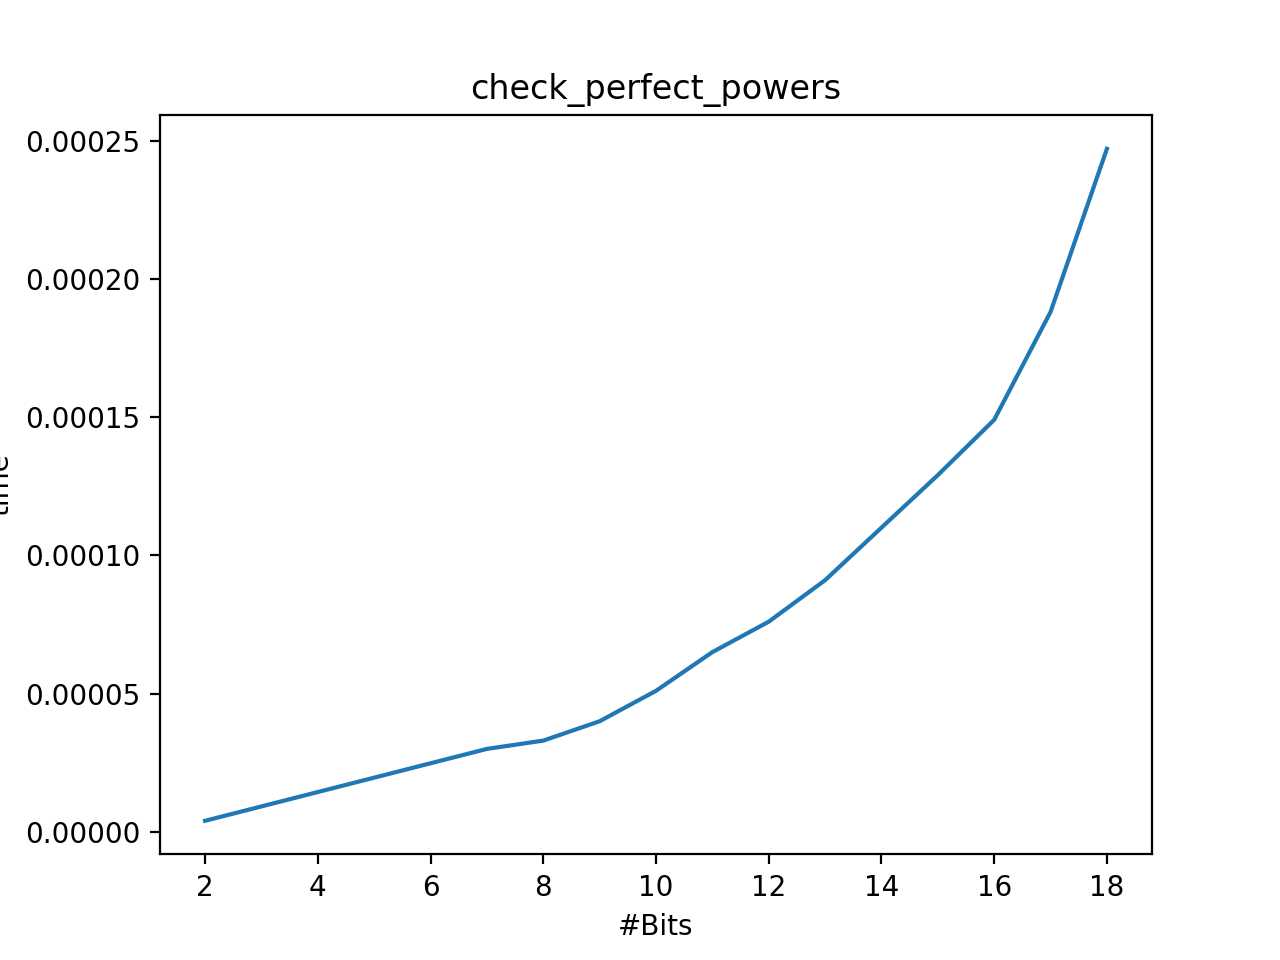
\includegraphics[width=8cm]{plots/pp.png}
\centering
\caption{Laufzeit des Potenz-Prüfung Algorithmus}
\end{figure}

Man kann nun empirisch zeigen, dass der Algorithmus korrekt ist, indem man Teiler $a $ von $n$ sucht und die Potenzen $a^b$ dieser ausrechnet, bis $n = a^b$. Die letzte Spalte der Tabelle \ref{table:1} bezeichnet $a^b$. Diese Werte können z.B. mit WolframAlpha geprüft werden. 


\newpage

\subsubsection{Experiment 2: Die Suche nach einem geeigneten $r$}
Einer der Hauptschritte des AKS-Algorithmus ist der zweite Schritt. Im zweiten Schritt wird nach einem geeinigten $r$ gesucht, sodass $o_r(n) > log^2 n$. Dies passiert durch ausprobieren von mehreren $r$ Werten. In Lemma \ref{limit_of_r} wurde gezeigt, dass dieses $r$ existiert, es wurde außerdem gezeigt, dass $r \leq log^5 n$.  
\begin{table}[h!]
\centering
\begin{tabular}{ |p{3cm}||p{3cm}|p{3cm}|p{3cm}|  }
 \hline
 \multicolumn{4}{|c|}{Laufzeituntersuchung} \\
 \hline
 Zahl & Inputgröße &Ergebnis&Zeit in s\\
 \hline
 7   & 3    &5&   $0.000032$\\
 41&   6  & 41   &$0.00038$\\
 771 &10 & 3&  $0.0001$\\
 6991    &13 & 149&  $0.02306$\\
 462975&   19  & 3&$ 0.0027$\\
 3875741& 22  & 443   &$1.512932$\\
 294024210& 29  & 2&$0.022265$\\
 \hline
\end{tabular}
 \caption{Laufzeituntersuchung des zweiten Schritts.}
\label{table:2}
\end{table}

Obige Tabelle \ref{table:2} zeigt, dass das geeignete $r$ auch für große Zahlen relativ schnell bestimmt werden kann. Es ist jedoch auffällig, dass der Algorithmus mehr zeit gebraucht hat um das geeignete $r$ für eine 22 Bit Zahl (3875741) zu finden, als für eine 29 Bit Zahl (294024210). Das liegt aber daran, dass der Algorithmus bei 294024210 weniger Zahlen ausprobieren musste.

Die polynomielle Laufzeit des 2. Schritts lässt sich auch am besten mit einer Grafik illustrieren:
\begin{figure}[h]
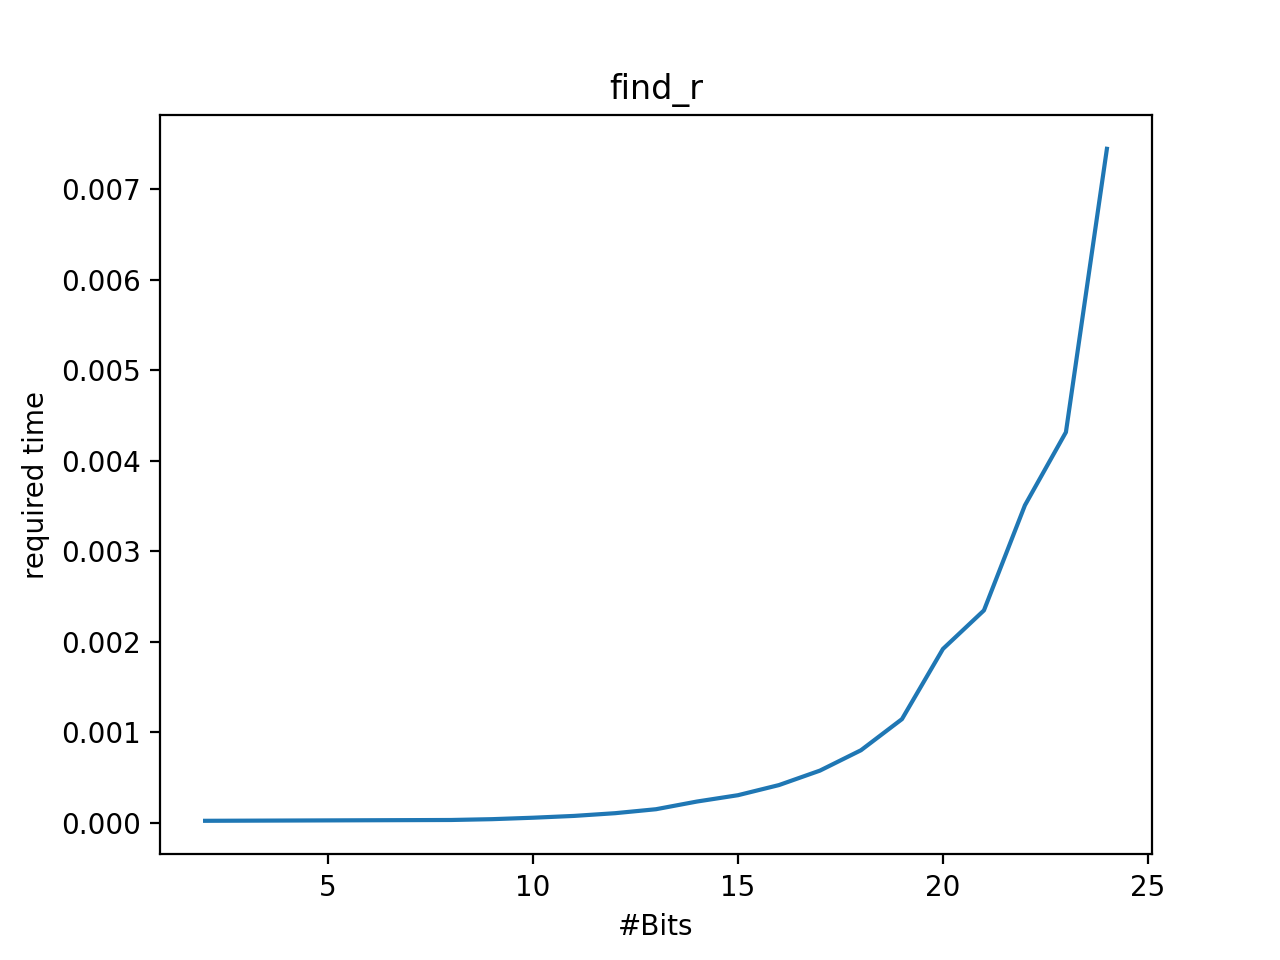
\includegraphics[width=8cm]{plots/findR.png}
\centering
\caption{Laufzeit von Schritt 2}
\end{figure}


\newpage

\subsubsection{Experiment 3: Laufzeit des AKS-Algorithmus}
In diesem Experiment wurde die Laufzeit des AKS-Algorithmus für mehrere bekannte Primzahlen gemessen\footnote{$\,$ Für die Primzahlen siehe \url{http://compoasso.free.fr/primelistweb/page/prime/liste_online_en.php} und \url{https://en.wikipedia.org/wiki/Largest_known_prime_number}.}. Es wurden auch bekannte zusammengesetzte Zahlen eingegeben, um die Korrektheit des Algorithmus zu testen. Diese sind aber nicht in der Laufzeit enthalten, da sie den schlechtestmöglichen Fall nicht darstellen.
\begin{table}[h!]
\centering
\begin{tabular}{ |p{3cm}||p{3cm}|p{3cm}|p{3cm}|  }
 \hline
 \multicolumn{4}{|c|}{AKS-Algorithmus} \\
 \hline
 Zahl & Inputgröße &Ergebnis&Zeit in s\\
 \hline
 49   & 6    &False&   $8.5 \cdot 10^{-5}$\\
 233&   8  & True   &$0.063$\\
 12923 &14 & True&  $0.302$\\
 131071    &17 & True&  $1.006$\\
 3875741& 22  & True   &$2.9943$\\
 38890279& 26  & True& $7.890$\\
 2147483647&   31  & True& $43.54$\\
 90552556447&   37  & False& $18.781$\\
 140141183298&   38  & False& $0.019$\\
 147763360000&   38  & False& $0.000065$\\
 170141183297& 38 & True& $119.432$\\
 \hline
\end{tabular}
 \caption{Laufzeituntersuchung des AKS-Algorithmus.}
\label{table:3}
\end{table}

\begin{figure}[h]
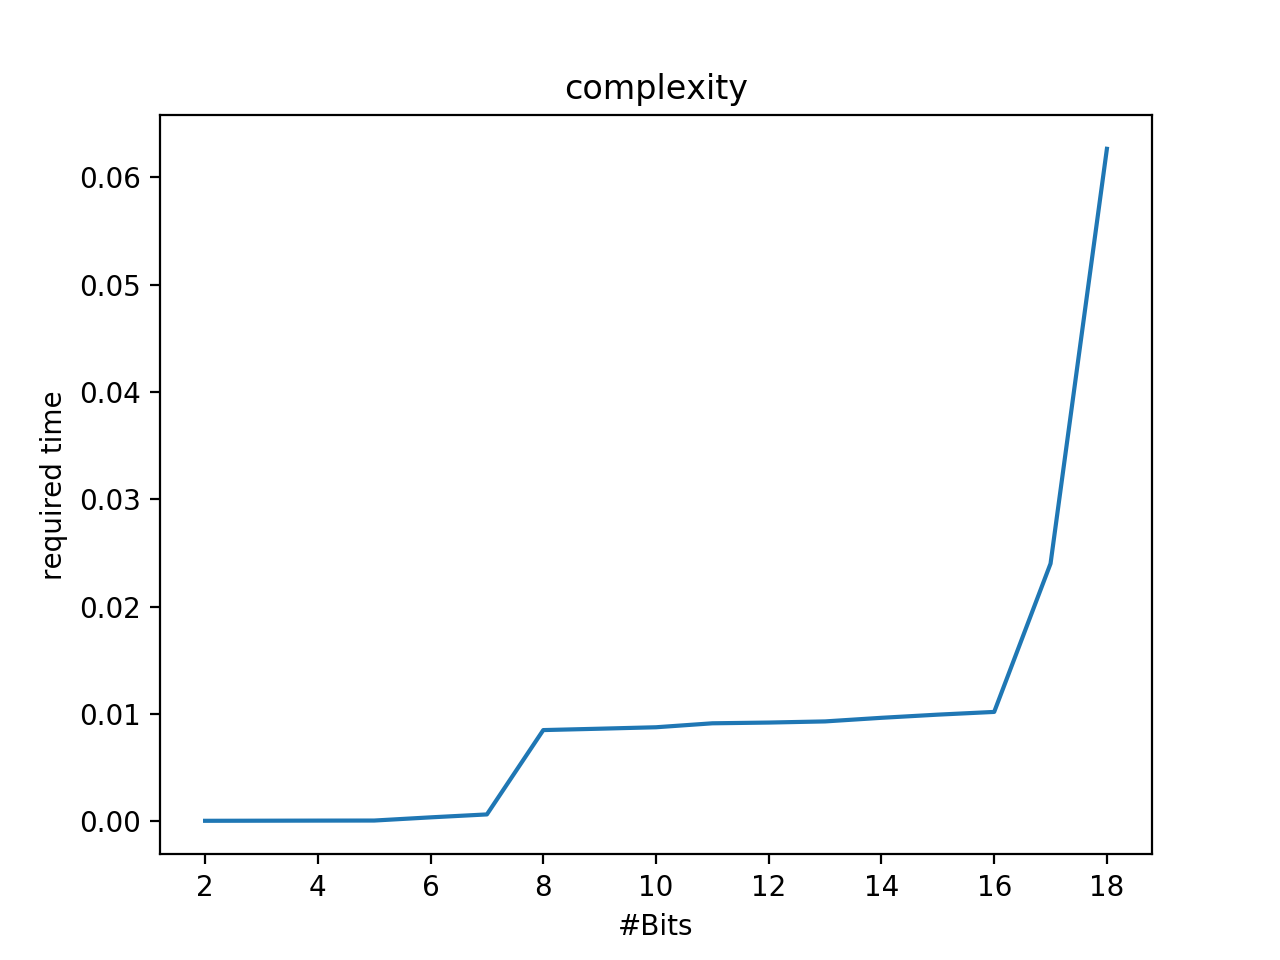
\includegraphics[width=8cm]{plots/aks.png}
\centering
\caption{Laufzeit des AKS-Primzahltests}
\end{figure}


% TODO: rewrite the whole passage !!
Tabelle \ref{table:3} zeigt deutlich, dass der zeitliche Aufwand des AKS-Algorithmus für Primzahlen kontinuierlich steigt, wenn die Eingabegröße größer wird. Das ist aber nicht unbedingt der Fall für zusammengesetzte Zahlen, da es zusammengesetzte Zahlen gibt, die schon im ersten Schritt des Algorithmus identifiziert werden, da sie Potenzen sind, ein Beispiel dafür wäre die Zahl 147763360000 mit der Inputgröße 38. Für 147763360000 hat der Algorithmus $6.5 \cdot 10^{-5}$ s gebraucht, und das ist wesentlich weniger als die gemessene Zeit für 90552556447 mit Inputgröße 37.

Aus dieser Beobachtung kann man nun auf die im Einleitung dieses Kapitels gestellte Frage beantworten. Der AKS-Algorithmus liefert die schnellste Antwort(ja oder nein), wenn die Zahl aus der Menge $M_1$ ist. Das liegt daran, dass solche Zahlen im ersten Schritt identifiziert werden, das heißt in $O(log^3 n)$. Es gibt jedoch zusammengesetzte Zahlen, die, im dritten(Zahlen aus $M_2$) oder im fünften Schritt(Zahlen aus $M_3$) identifiziert werden. Für diese Zahlen ist der maximale Aufwand $O^{\sim}(log^{21/2}n)$.\footnote{$\,$ Diese sind Zahlen, die in der Schleife des 5. Schritts identifiziert werden.} Während Primzahlen entweder im vierten oder im sechsten Schritt identifiziert werden, das bedeutet entweder in $O^{\sim}(log^7n)$ oder $O^{\sim}(log^{21/2}n)$. Daraus kann man folgern, dass Primzahlen und zusammengesetzte Zahlen im schlimmsten Fall nach $O^{\sim}(log^{21/2}n)$ erkannt werden. Im besten Fall kann der AKS-Algorithmus eine schnellere Antwort liefern, wenn die Zahl zusammengesetzt ist. Daher lautet die Antwort auf die Frage: der AKS-Algorithmus liefert für zwei gleich große Zahlen(eine Primzahl und eine zusammengesetzte Zahl) im Durchschnitt eine schnellere Antwort\footnote{$\,$ Schneller im Sinne von der Anzahl an Schritte.}, wenn die Zahl zusammengesetzt ist. Das heißt, dass die durchschnittliche Laufzeit für zusammengesetzte Zahlen kleiner als die durchschnittliche Laufzeit für Primzahlen ist.      

\subsubsection{Experiment 4: AKS vs naiver Primzahltest}
In der Einführung wurde ein Algorithmus erwähnt, der das Primalitätsproblem in $\Omega(\sqrt{n})$ löst. Allerdings hat dieser Algorithmus eine exponentielle Laufzeit. Der AKS-Algorithmus hat eine polynomielle Laufzeit, und ist somit schneller als der naive Primzahltest(engl. brute-force primality test). In diesem Experiment wurden die Laufzeiten beider Algorithmen bis zur Inputgröße $37$ verglichen.  

Zur Untersuchung der Laufzeit beider Algorithmen als Primzahltest werden bewusst nur Primzahlen als Eingabewerte herangezogen. Das liegt einerseits daran, dass diese den schlechtest möglichen Fall beider Algorithmen darstellt. Andererseits ist oft der Fall, dass der AKS-Algorithmus für zusammengesetzte Zahlen aus $M_1$ das Ergebnis  schnell liefern kann.\newline\footnote{. Dadurch soll ein Verglich zwischen der Potenz-Prüfung und dem naiven Algorithmus vermieden werden.}

\begin{table}[h!]
\centering
\begin{tabular}{ |p{3cm}||p{3cm}|p{3cm}|p{3cm}|  }
 \hline
 \multicolumn{4}{|c|}{AKS vs Naive} \\
 \hline
 Zahl & Inputgröße  & AKS [in s] &Naive [ in s]\\
 \hline
 8191   & 13    &0.319566&   0.0006\\
 131071&   17  & 0.990821   &0.01\\
 524287 &19 &  1.5811& 0.04\\
 38757413    &26 & 7.556&   2.933\\
 2147483647& 31  & 42.58   &162.3\\
 2547587681& 32  &  43.902&  187.876\\
 17014120163&   34  & 86.073& 1275.286\\
 90552556889&   37  & 97.769072& 6732.12\\

 \hline
\end{tabular}
 \caption{AKS vs naiver Primzahltest.}
\label{table:4}
\end{table}


Obige Tabelle macht deutlich, dass der AKS-Primzahltest eine bessere asymptotische Laufzeit als der naive Primzahltest hat.

Man kann nun die Werte aus Tabelle \ref{table:4} in einer Grafik darstellen. 

\begin{figure}[h]
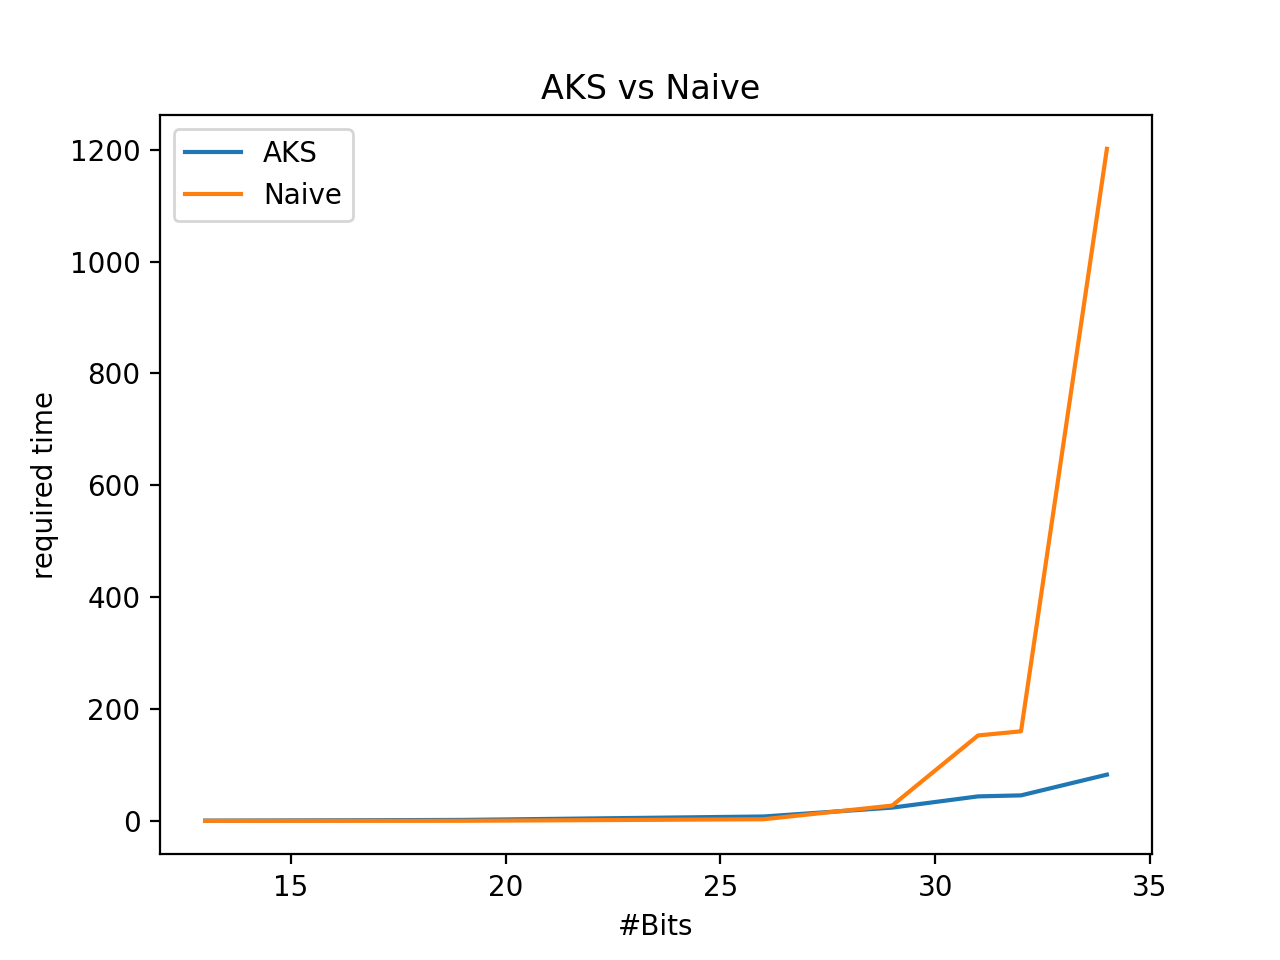
\includegraphics[width=8cm]{plots/aksVsNaive.png}
\centering
\caption{Laufzeit des AKS-Algorithmus im Vergleich zum naiven Algorithmus}
\label{plot_aks_naive}
\end{figure}

Grafik \ref{plot_aks_naive} zeigt deutlich, dass der AKS-Algorithmus bei Inputgröße $37$ in unter $200 \, s$ eine Antwort geliefert hat, während der naive Algorithmus mehr als $6500 \, s(> 1.5 h)$ brauchte.


\begin{figure}[h]
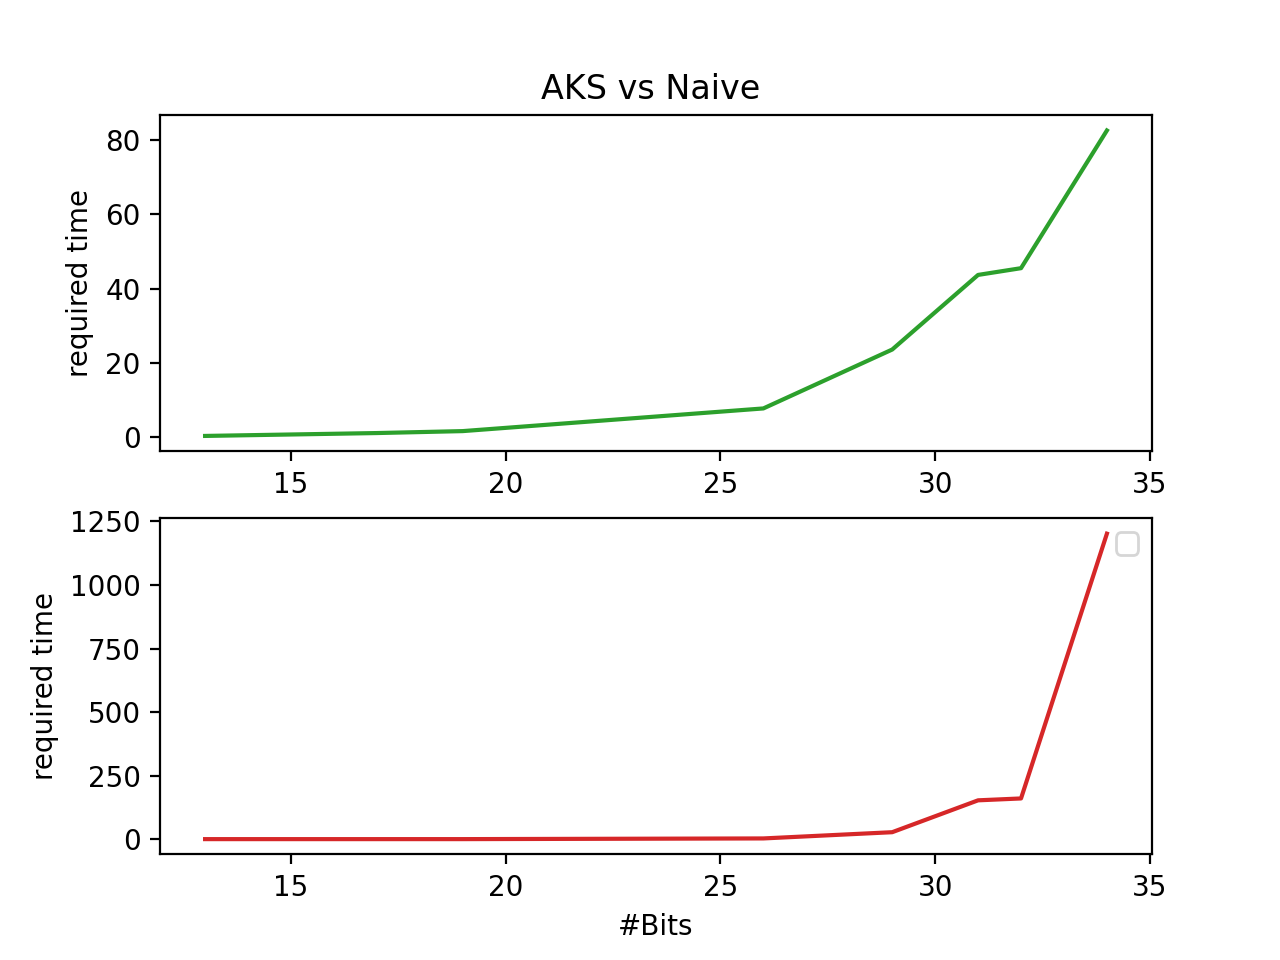
\includegraphics[width=8cm]{plots/aksVsNaiveSubPlots.png}
\centering
\caption{Laufzeit des AKS-Algorithmus(grün) im Vergleich zum naiven Algorithmus(rot)}
\end{figure}

\section{Zusammenfassung}


%%%%%%%%%%%%%%%%%%%%%%%%%%%%
%% Literaturverzeichnis wird 
%% automatisch eingefügt
%%%%%%%%%%%%%%%%%%%%%%%%%%%%
\clearpage
\lhead{}
\printbibliography
\addcontentsline{toc}{section}{\bibname}


%%%%%%%%%%%%%%%%%%%%%%%%%%%%
%% Anhang (optional) 
%%%%%%%%%%%%%%%%%%%%%%%%%%%%
\clearpage
\appendix
\section{Algorithmenverzeichnis}
% check_perefect_powers
\begin{algorithm}[H]
\SetAlgoLined
\KwIn{$n \in \mathbb{N}, n \geq 2$.}
\begin{enumerate}
\item $a, \, b, \, c, \, m$

\item $ b = 2$.

\item \textbf{while} $2^b \leq n$ \textbf{repeat}

\item $\: \: \: \: $ $a = 1, \, c = n $

\item $\: \: \: \: $ \textbf{while} $c - a \geq 2$ \textbf{repeat}

\item $\: \: \: \: \: \: \: \: \:$ $ m = \lfloor (a + c)/2 \rfloor$

\item $\: \: \: \: \: \: \: \: \:$ $ p = min\{m^b,n+1\}$

\item $\: \: \: \: \: \: \: \: \:$ \textbf{if} $ p = n$ \textbf{return} True.

\item $\: \: \: \: \: \: \: \: \:$ \textbf{if} $p < n$

\item $\: \: \: \: \: \: \: \: \: \: \: \: \: \:$  $ a = m$

\item $\: \: \: \: \: \: \: \: \:$ \textbf{else}

\item $\: \: \: \: \: \: \: \: \: \: \: \: \: \:$  $c = m$

\item $\: \: \: \: $ $b = b + 1$

\item \textbf{return} False


\end{enumerate}
\caption{Potenz-Prüfung}
\label{appendix:potenz}
\end{algorithm}

% fast expo algorithm
\begin{algorithm}[H]
\SetAlgoLined
\KwIn{$a \in M, n \geq 0$}
\begin{enumerate}
    \item $u = n$.
    \item $s = a$.
    \item $c = 1$.
    \item \textbf{while} $u \geq 1$ \textbf{repeat}
    \item $\; \: \: \;$ \textbf{if} $u \, mod \, 2 \neq 0$ \textbf{then}
       $ \; c = c \circ s$
     \item $\; \: \: \;$ $s = s \cdot \, mod \, M$
     \item $\; \: \: \;$ $ u = u \, div \, 2$
     \item \textbf{return $c$}
\end{enumerate}
 \caption{Schnelle modulare Exponentiation}
 \label{appendix:fast_expo}
\end{algorithm}

%%%%%%%%%%%%%%%%%%%%%%%%%%%%
%% Eidesstattliche Erklärung
%% muss angepasst werden 
%% in Erklaerung.tex
%%%%%%%%%%%%%%%%%%%%%%%%%%%%
\newpage
\begin{otherlanguage}{ngerman}
\thispagestyle{empty}
\section*{Eidesstattliche Erklärung}
\thispagestyle{empty}
Hiermit versichere ich, die vorliegende Arbeit selbstständig verfasst und keine anderen als die angegebenen Quellen und Hilfsmittel benutzt sowie die Zitate deutlich kenntlich gemacht zu haben.
\newline
\vspace{4\baselineskip}\\
Leipzig, den \today \hfill Salman Salman 
\vspace{4\baselineskip}\\
\end{otherlanguage}

\end{document}
